% You should title the file with a .tex extension (hw1.tex, for example)
\documentclass[11pt]{article}

\usepackage{amsmath}
\usepackage{amssymb}
\usepackage{fancyhdr}
\usepackage{graphicx}
\usepackage{subcaption}
\usepackage{multirow}
\usepackage{bbm}
\usepackage{bm}
\usepackage{wasysym}
\usepackage{hyperref}
\usepackage{makecell}

\hypersetup{
    colorlinks=true,
    linkcolor=blue 
    }

\oddsidemargin0cm
\topmargin-2cm     %I recommend adding these three lines to increase the 
\textwidth16.5cm   %amount of usable space on the page (and save trees)
\textheight23.5cm  

\newcommand{\question}[2] {\vspace{.25in} \hrule\vspace{0.5em}
\noindent{\bf #1: #2} \vspace{0.5em}
\hrule \vspace{.10in}}
\renewcommand{\part}[1] {\vspace{.10in} {\bf (#1)}}

\newcommand{\myname}{Joao Vitor Dias Monteiro}
\newcommand{\myandrew}{jmonteir@andrew.cmu.edu}
\newcommand{\myhwnum}{5}

\newcommand{\bW}{\bm{W}}
\newcommand{\bx}{\bm{x}}
\newcommand{\bp}{\bm{p}}
\newcommand{\bA}{\bm{A}}
\newcommand{\bb}{\bm{b}}
\newcommand{\bH}{\bm{H}}
\newcommand{\bP}{\bm{P}}
\newcommand{\bC}{\bm{C}}
\newcommand{\bh}{\bm{h}}
\newcommand{\bK}{\bm{K}}
\newcommand{\bzero}{\bm{0}}
\newcommand{\bX}{\bm{X}}
\newcommand{\bR}{\bm{R}}
\newcommand{\bI}{\bm{I}}
\newcommand{\real}{\mathbb{R}}
\newcommand{\bF}{\bm{F}}
\newcommand{\bE}{\bm{E}}
\newcommand{\bt}{\bm{t}}
\newcommand{\bl}{\bm{l}}
\newcommand{\bS}{\bm{S}}
\newcommand{\bM}{\bm{M}}
\newcommand{\bw}{\bm{w}}



\setlength{\parindent}{0pt}
\setlength{\parskip}{5pt plus 1pt}
 
\pagestyle{fancyplain}
\lhead{\fancyplain{}{\textbf{HW\myhwnum}}}      % Note the different brackets!
\rhead{\fancyplain{}{\myname\\ \myandrew}}
\chead{\fancyplain{}{16-720}}

\begin{document}

\medskip                        % Skip a "medium" amount of space
                                % (latex determines what medium is)
                                % Also try: \bigskip, \littleskip

\thispagestyle{plain}
\begin{center}                  % Center the following lines
{\Large CMU 16-720: Homework \myhwnum} \\
\myname \\
\myandrew \\
%Recitation: Your recitation section \\
December 4, 2022 \\
\end{center}

\question{Q1.1}{Prove that softmax is invariant to translation. Oftenr we use $c = - max\;x_i$. Why is that a good idea?}

$$
softmax(x_i) = \frac{e^{x_i}}{\sum_{j=1}^n e^{x_j}} = \frac{e^{x_i}}{\sum_{j=1}^n e^{x_j}} \times \frac{e^{c}}{e^{c}} = \frac{e^{x_i+c}}{\sum_{j=1}^n e^{x_j+c}} = softmax(x_i+c)
$$

Often $c = - max\;x_i$ is used for the purpose of numerical stability since in that case $e^{x_j+c}$ will be at most one, thus guaranteeing the denominator will not
have large values due to the exponentials.

\clearpage

\question{Q1.2}{What is the range of $softmax(x_i)$? What is $\sum_{i=1}^N softmax(x_i)$?}

\begin{itemize}
    \item The range of $softmax(x_i)$ is between 0 and 1. The sum of all $softmax(x_i)$ terms is 1. 
    \item One could say that ``softmax takes an arbitrary real values vector and turns it into a vector of numbers between zero and one''.
    \item $s_i = e^{x_i}$ maps $x_i$ into a positive number , $S = \sum s_i$ computes the sum of all $s_i$ and $softmax(x_i) = (1/S)s_i$ maps $s_i$ to a number between 0 and 1.
\end{itemize}

\clearpage

\question{Q1.3}{Show that multi-layer neural networks without a non-linear activation function are equivalent to linear regression.}
Without loss of generality, consider a neural network with 3 layers:

$$
\hat{y} = h_3(\bW_3h_2(\bW_2h_1(\bW_1x+\bb_1)+\bb_2)+\bb_3)
$$
where $h_i$ is the activation function, $\bW \in \mathbb{R}^{k_i \times k_{i-1}}$ is the weight matrix, $\bb \in \mathbb{R}^{k_i}$ is the bias term,
$k_i$ is the number of nodes and subscript $i$ means that all of these are associated with the i-th layer. Lastly, $x \in \mathbb{R}^{k_0}$ is the input features and $\hat{y}$ the corresponding prediction
by this multilayer neural network.

Now, let $h_i$ be a linear function, that is 
$$
h_i(z) = \bM_i z
$$
where $\bM_i \in \mathbb{R}^{k_i \times k_i}$. Notice that 

$$
h_1(\bW_1x+\bb_1) = \bM_1(\bW_1x+\bb_1) = \bM_1\bW_1x + \bM_1\bb_1 = \bW_1^{*}x+\bb_1^{*}
$$

$$
h_2(\bW_2h_1(\bW_1x+\bb_1)+\bb_2) = \bM_2(\bW_2\bW_1^{*}x+\bW_2\bb_1^{*}+\bb_2) = \bW_2^{*}x+\bb_2^{*}
$$

$$
\hat{y} = h_3(\bW_3(\bW_2^{*}x+\bb_2^{*})) = \bM_3(\bW_3\bW_2^{*}x+\bW_3\bb_2^{*}+\bb_3) = \bW_3^{*}x+\bb_3^{*}
$$

Therefore $\hat{y}$ is a linear transformation of $x$ thus proving that if $h_i$'s are linear activation functions the neural network
becomes a linear regression.

\clearpage

\question{Q1.4}{Given the sigmoid function $\sigma(x)= \frac{1}{1+e^{-x}}$, derive the gradient of the sigmoid function and show that it can be written as a function of 
$\sigma(x)$.}

$$
\begin{aligned}
    \frac{d}{dx}\sigma(x) &= \frac{0\times(1-e^{-x}) - 1\times(-e^{-x})}{(1+e^{-x})^2} \\
                          &= \left(\frac{e^{-x}}{1+e^{-x}}\right) \times \frac{1}{1+e^{-x}}\\
                          &= \left(1 - \frac{1}{1+e^{-x}}\right) \times \frac{1}{1+e^{-x}} \\
                          &= [1-\sigma(x)]\sigma(x)
\end{aligned}
$$
\clearpage

\question{Q1.5}{Given $y = Wx +b$ and the gradient of some loss $J$ with respect $y$, show how to get $\frac{\partial J}{\partial W}$, $\frac{\partial J}{\partial x}$ and $\frac{\partial J}{\partial b}$.}

By using chain rule we can get
$$
\frac{\partial J}{\partial W_{ij}} = \left(\frac{\partial J}{\partial y}\right) \frac{\partial y}{\partial W_{ij}} = \delta_i x_j
$$
Therefore, 
$$
\frac{\partial J}{\partial W} = 
\begin{bmatrix}\delta_1 x_1 & \delta_1 x_2 & \cdots & \delta_1 x_d \\ 
             \delta_2 x_1 & \delta_2 x_2 & \cdots & \delta_2 x_d  \\
              \vdots & \vdots & \vdots & \vdots \\
              \delta_k x_1 & \delta_k x_2 & \cdots & \delta_k x_d\end{bmatrix} = \delta x^{T}
$$

Similarly, 

$$
\frac{\partial J}{\partial x} = \left[\left(\frac{\partial J}{\partial y}\right)^T \frac{\partial y}{\partial x}\right]^{T} = \left(\delta^TW\right)^T = W^T\delta
$$

and

$$
\frac{\partial J}{\partial b} = \left[\left(\frac{\partial J}{\partial y}\right)^T \frac{\partial y}{\partial b}\right]^{T} = \left(\delta^T I_k\right)^T = \delta
$$
where $I_k$  is a $k\times k$ identity matrix.

\clearpage

\question{Q1.6}{Various questions about vanishing gradient problem, and comparison between tanh and sigmoid}

\begin{enumerate}
    \item The gradient of sigmoid activation function is a number between 0 and 1. Thus, in a deep neural networks with many layers the gradient in the backpropagation update will be the product of many numbers
     between 0 and 1 which leads to the vanish gradient problem (i.e. gradient becoming close to zero).
    \item The sigmoid function ranges between 0 and 1, while the tanh function ranges between -1 and 1. We might prefer tanh because tanh is symmetric around 0.
    \item Because the derivative of tanh around zero (where the normalized input data would be) is larger than the derivative of the sigmoid.
    \item $tanh(x) = \frac{1-e^{-2x}}{1+e^{-2x}} = (1-e^{-2x})\frac{1}{1+e^{-2x}} = (1-e^{-2x})\sigma(2x) = \sigma(2x) - \sigma(2x)(1+e^{-2x}-1) = \sigma(2x) - \sigma(2x)\left(\frac{1}{\sigma(2x)}-1\right) = 2\sigma(2x)-1$

\end{enumerate}

\clearpage

\question{Q2.1.1}{Why is it not a good idea to initialize a network with all zeros? If you imagine that every layer has weights and biases, what can a zero-initialized network
output after training?}
Because when initialize a network with all zeros different units (i.e. neurons) will have the same update in the gradient during the backpropagation. Consequently, the weights and biases associated with those
distinct units will be the same, and thus reducing considerably the representation power of the neural network model.

\clearpage

\question{Q2.1.2}{Implement function initialize\_weights in python/nn.py. Include your code in the writeup.}

Figure \ref{fig:initialize_weights} shows the code snippet of the function initialize\_weights.
\begin{figure}[h!]
    \centering
    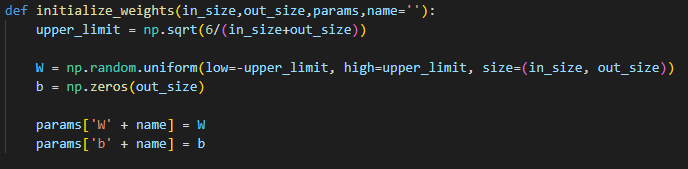
\includegraphics[width=0.65\textwidth]{figures/initialize_weights_snapshot.png}    
    \caption{Code snippet of the function initialize\_weights}
    \label{fig:initialize_weights}
\end{figure}

\clearpage
\question{Q.2.1.3}{Why do we initialize with random numbers? Why do we scale the initialization depending on layer size?}
We initialize a neural network with random numbers to break the symmetry between distinct units and avoid that distinct units have the same (or similar) update in the gradient during backpropagation and
consequently reducing the representation power of the neural network. 

The standard initialization (Equation 1 in the paper) causes the variance of the back-propagated gradient to be dependent on the layer. In particular, the variance of the back-propagated gradient gets
smaller as it is propagated downwards, and consequently there is more risk of having vanishing gradient problems. However, the authors found that such decreasing back-propagated gradients is not 
observed when scaling the initialization according to the layer size.

\clearpage
\question{Q2.2.1}{In python/nn.py implement function sigmoid. Include your code in the writeup.}

Figure \ref{fig:sigmoid} shows the code snippet of the function sigmoid.
\begin{figure}[h!]
    \centering
    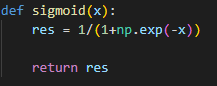
\includegraphics[width=0.35\textwidth]{figures/sigmoid_snapshot.png}    
    \caption{Code snippet of the function sigmoid}
    \label{fig:sigmoid}
\end{figure}


\clearpage
\question{Q2.2.2}{In python/nn.py implement the softmax function. Include your code in the writeup.}

Figure \ref{fig:softmax} shows the code snippet of the function softmax.
\begin{figure}[h!]
    \centering
    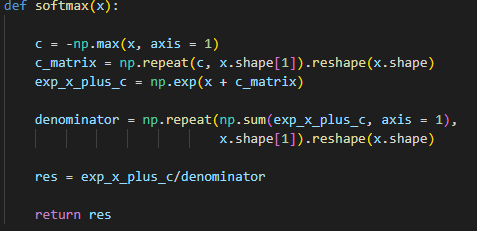
\includegraphics[width=0.55\textwidth]{figures/softmax_snapshot.png}    
    \caption{Code snippet of the function softmax}
    \label{fig:softmax}
\end{figure}

\clearpage
\question{Q.2.2.3}{In python/nn.py, implement the function compute\_loss\_and\_acc. Include your code in the writeup.}

Figure \ref{fig:loss} shows the code snippet of the function compute\_loss\_and\_acc.
\begin{figure}[h!]
    \centering
    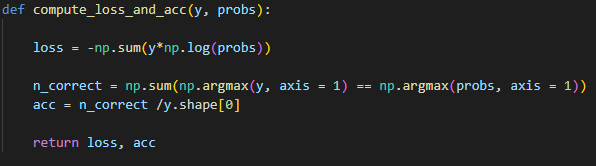
\includegraphics[width=0.55\textwidth]{figures/loss_snapshot.png}    
    \caption{Code snippet of the function compute\_loss\_and\_acc}
    \label{fig:loss}
\end{figure}

\clearpage
\question{Q2.3}{In python/nn.py, implement function backwards. Include your code in the writeup.}

Figure \ref{fig:backwards} shows the code snippet of the function backwards.
\begin{figure}[h!]
    \centering
    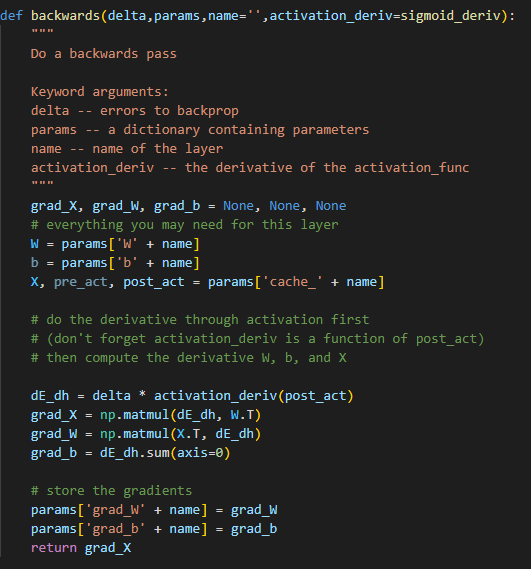
\includegraphics[width=0.55\textwidth]{figures/backwards_snapshot.png}    
    \caption{Code snippet of the function backwards}
    \label{fig:backwards}
\end{figure}

\clearpage

\question{Q2.4}{In python/nn.py implement function get\_random\_batches. In python/run\_q2.py, write a training loop that iterates over the batches, does
foward and backward propagation, and applies gradient update. Include your code in the writeup.}

Figure \ref{fig:batches} shows the code snippet of the function get\_random\_batches.
\begin{figure}[h!]
    \centering
    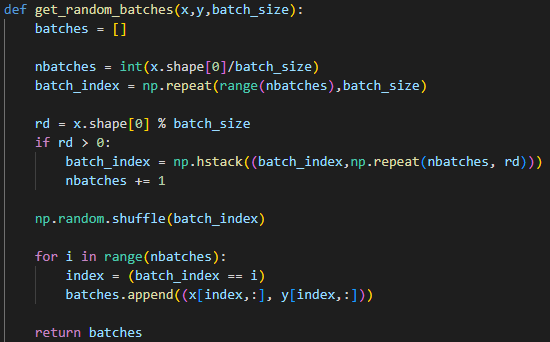
\includegraphics[width=0.45\textwidth]{figures/batches_snapshot.png}    
    \caption{Code snippet of the function get\_random\_batches}
    \label{fig:batches}
\end{figure}

Figure \ref{fig:forward_backward} shows the code snippet of the training loop (in python/run\_q2.py) that iterates over the batches, does
foward and backward propagation, and applies gradient update.
\begin{figure}[h!]
    \centering
    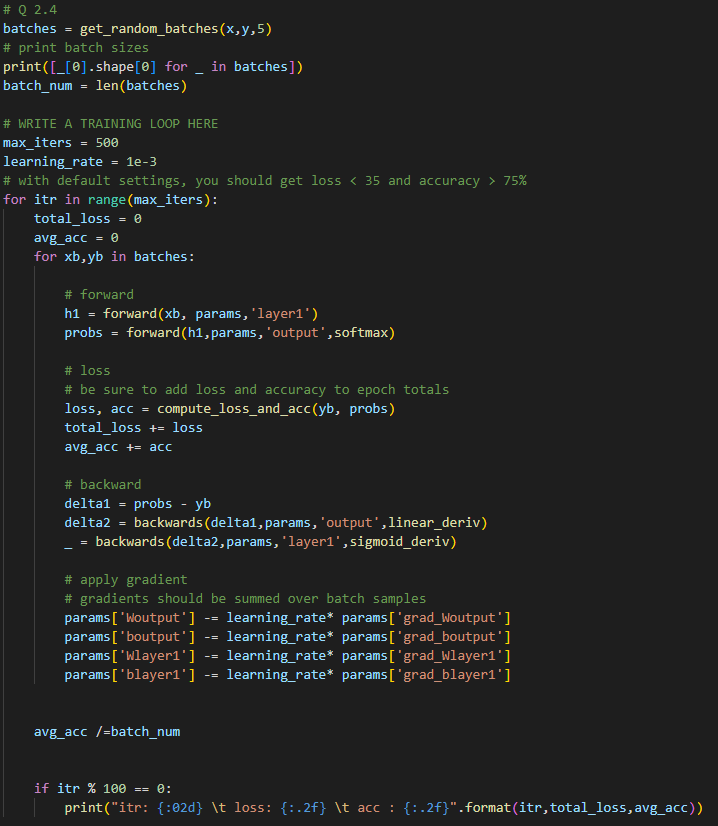
\includegraphics[width=0.55\textwidth]{figures/forward_backward_snapshot.png}
    \caption{Code snippet of the training loop (in python/run\_q2.py) that iterates over the batches, does
    foward and backward propagation, and applies gradient update.}
    \label{fig:forward_backward}
\end{figure}

\clearpage

\question{Q2.5}{In python/nn.py implement a numerical gradient checker. Include your code in the writeup.}

Figure \ref{fig:gradient_checker} shows the code snippet of the numerical gradient checker (in python/run\_q2.py).
\begin{figure}[h!]
    \centering
    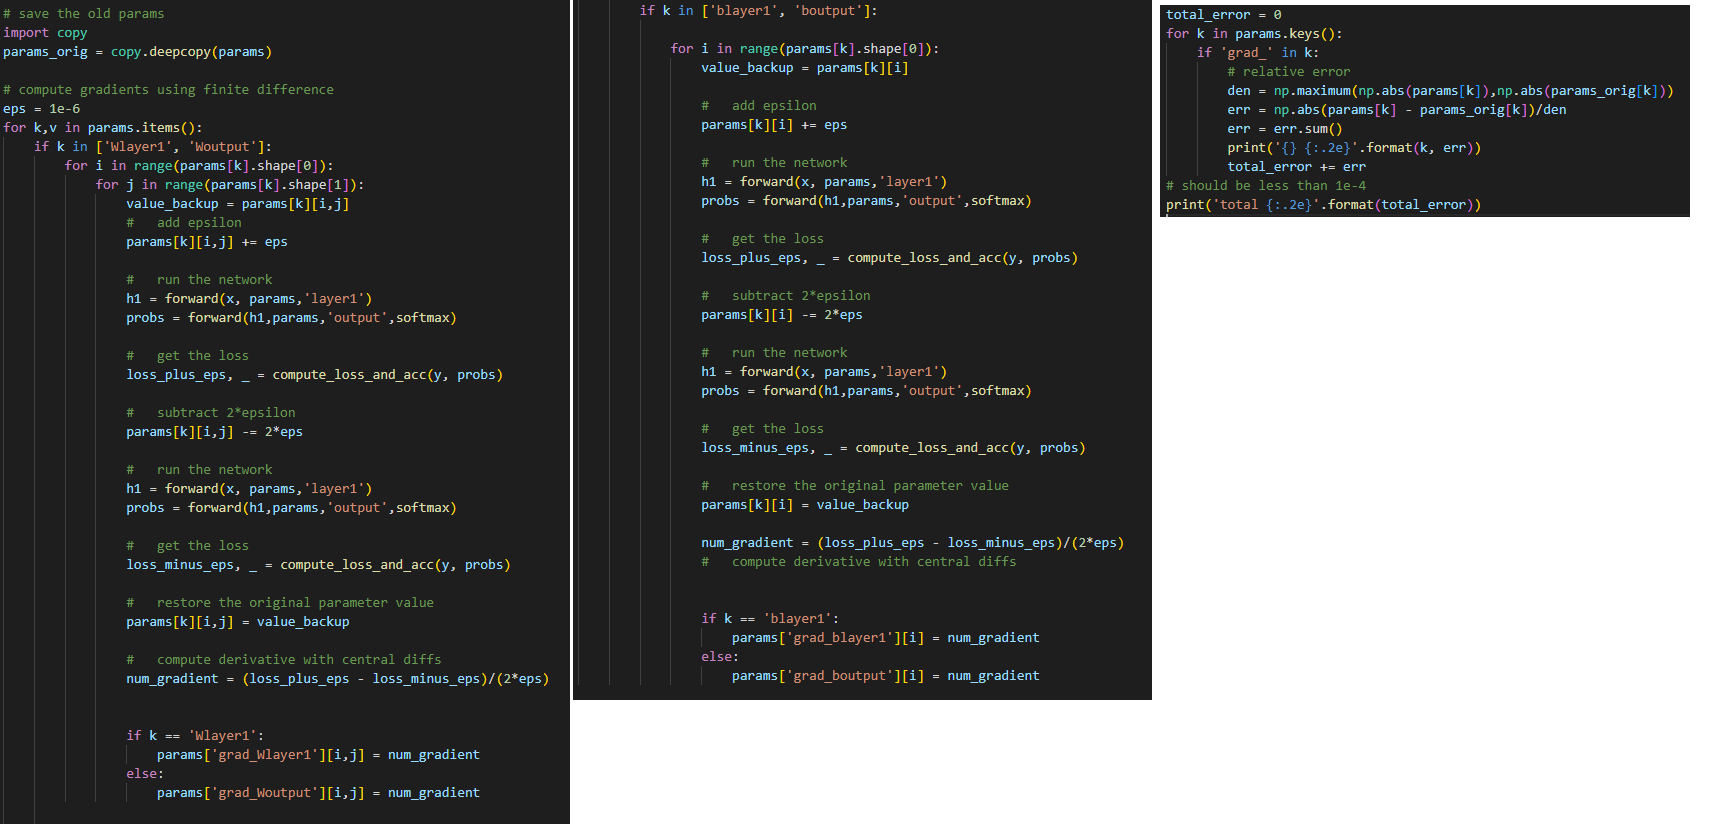
\includegraphics[width=0.95\textwidth]{figures/gradient_checker.png}
    \caption{Code snippet of the numerical gradient checker (in python/run\_q2.py).}
    \label{fig:gradient_checker}
\end{figure}

\clearpage
\question{Q3.1}{Train a network from scratch. Use a single hidden layer with
64 hidden units, and train for at least 50 epochs. The script will generate two plots: one
showing the accuracy on both the training and validation set over the epochs, and the other
showing the cross-entropy loss averaged over the data. Tune the batch size and learning rate
to get an accuracy on the validation set of at least 75\%. Include the plots in your writeup.}

I trained a neural network with a single hidden layer (64 hidden units) for 600 epochs. I used a batch size of 16 and learning rate 
equal to 0.001. The final validation accuracy was 77.4\%, and the final test accuracy was 78.3\%.  Figures \ref{fig:q_3_1} (a)-(b) show 
respectively the loss and accuracy over the epochs, both for training and validation sets. 

\begin{figure}[h!]
    \centering
    \begin{tabular}{cccc}
    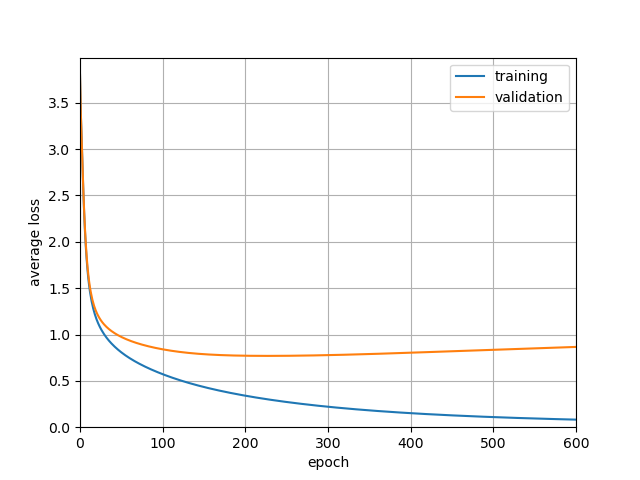
\includegraphics[width=0.45\textwidth]{figures/q_3_1_loss.png}  &  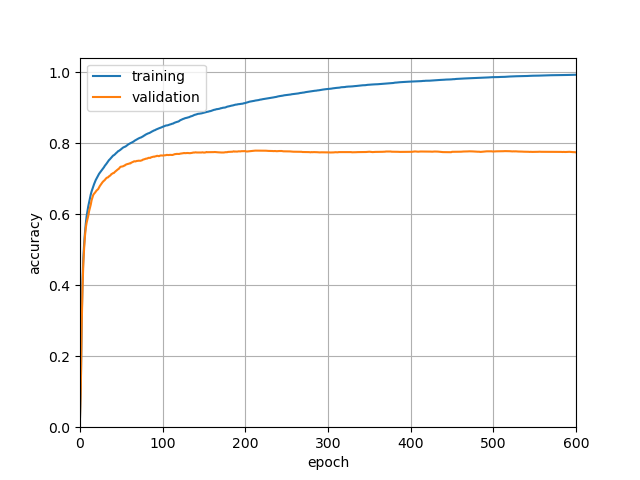
\includegraphics[width=0.45\textwidth]{figures/q_3_1_accuracy.png}  \\  
    \textbf{(a)} Loss by epoch step & \textbf{(b)} Accuracy by epoch step\\ [6pt] 
    \end{tabular}
    \caption{Loss and accuracy over the epochs for training (blue lines) and validation (orange lines) datasets}\label{fig:q_3_1}
\end{figure} 



\clearpage

\question{Q3.2}{Use the script to train three networks, one with your tuned learning rate, one with 10 times that learning rate, and one with one tenth that learning
rate. Include all six plots in your writeup. Comment on how the learning rates affect the training, and report the final accuracy of the best network on the test set.}


Table \ref{tab:acc_comparison} shows the validation and test accuracies after training the same neural network architecture 
for 600 epochs using distinct learning rates: 0.0001, 0.001 and 0.01. The best test accuracy was observed when using the 
learning rate 0.001, while the worst test accuracy was observed when using tthe learning rate 0.0001.

\begin{table}[!h]
\centering
\caption{Validation and test accuracies after training same neural network architecture for 600 epochs using distinct learning rates: 0.0001, 0.001 and 0.01}
\label{tab:acc_comparison}
    \begin{tabular}{|c|ccc|}
    \hline
               & \multicolumn{3}{c|}{Learning Rate}                                  \\ \hline
               & \multicolumn{1}{c|}{0.0001} & \multicolumn{1}{c|}{0.001} & 0.01  \\ \hline
    Validation & \multicolumn{1}{c|}{75.3\%}  & \multicolumn{1}{c|}{77.4\%} & \% 75.3\%\\ \hline
    Test       & \multicolumn{1}{c|}{75.4\%}  & \multicolumn{1}{c|}{78.3\%} & \% 75.7\%\\ \hline
    \end{tabular}
\end{table}


Figures \ref{fig:q_3_2} (a)-(f) show loss and accuracy over the epochs for training (blue lines) and validation (orange lines) datasets for three different 
learning rates: 0.0001, 0.001 and 0.01. The higher the training rate the more rapidly was the drop in the loss in the earlier epochs (both training and validation). Similarly, 
the higher the learning rate the faster was the increase in accuracy (both training and validation). However, as seen in Figure \ref{fig:q_3_2}(e), if  learning rates are too large then the 
gradient descent algorithm can jump over areas with lower loss function. 

\begin{figure}[h!]
    \centering
    \begin{tabular}{cccc}
    
    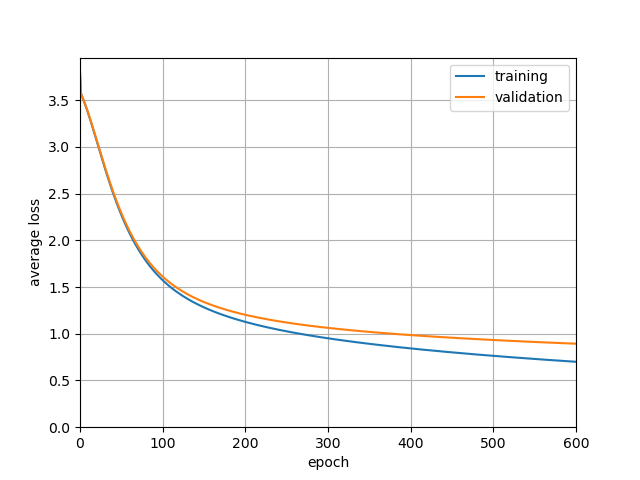
\includegraphics[width=0.45\textwidth]{figures/q_3_2_loss_one_tenth.png}  &  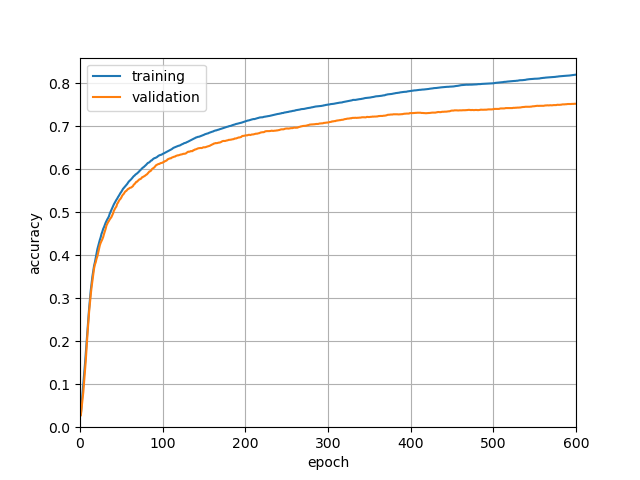
\includegraphics[width=0.45\textwidth]{figures/q_3_2_accuracy_one_tenth.png}  \\  
    \textbf{(a)} Loss by epoch step - learning rate: 0.0001 & \textbf{(b)} Accuracy by epoch step - learning rate: 0.0001\\ [6pt] 

    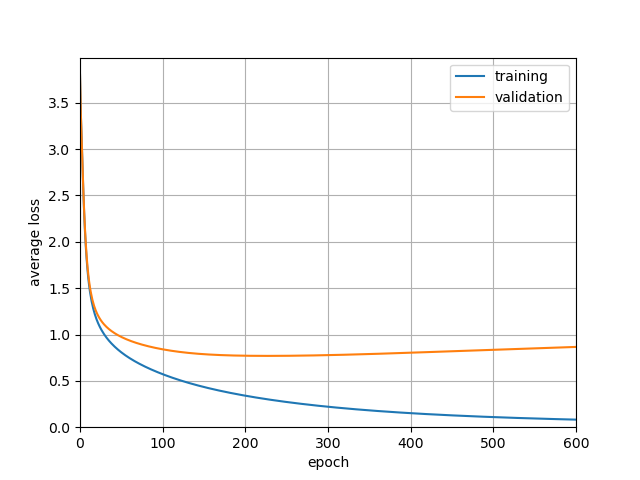
\includegraphics[width=0.45\textwidth]{figures/q_3_1_loss.png}  &  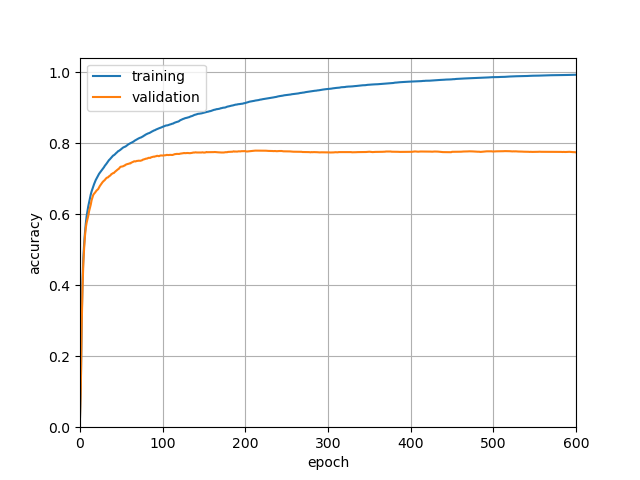
\includegraphics[width=0.45\textwidth]{figures/q_3_1_accuracy.png}  \\  
    \textbf{(c)} Loss by epoch step - learning rate: 0.001 & \textbf{(d)} Accuracy by epoch step - learning rate: 0.001\\ [6pt] 

    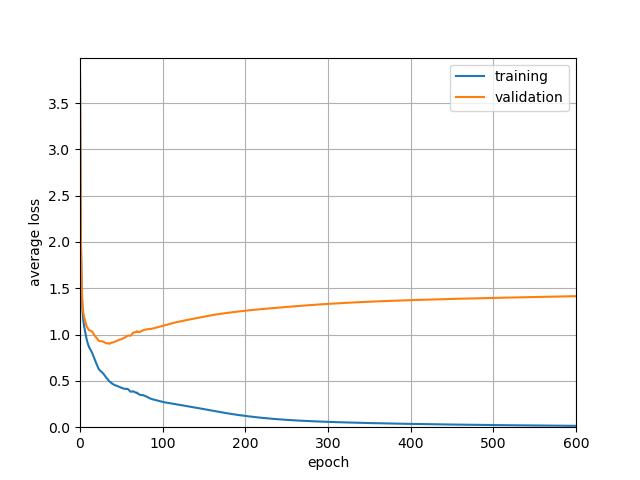
\includegraphics[width=0.45\textwidth]{figures/q_3_2_loss_10times.png}  &  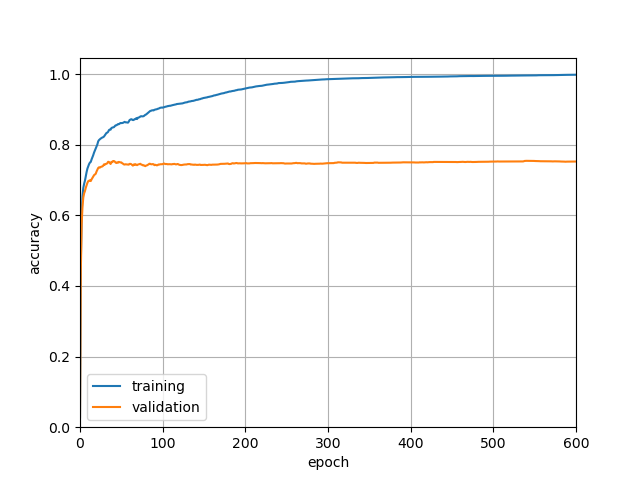
\includegraphics[width=0.45\textwidth]{figures/q_3_2_accuracy_10times.png}  \\  
    \textbf{(e)} Loss by epoch step - learning rate: 0.01 & \textbf{(e)} Accuracy by epoch step - learning rate: 0.01\\ [6pt] 

    \end{tabular}
    \caption{Loss and accuracy over the epochs for training (blue lines) and validation (orange lines) datasets for three different learning rates: 0.00001 (a, b), 0.0001 (c, d) and 0.001 (e, f)}\label{fig:q_3_2}
\end{figure} 

\clearpage

\question{Q3.3}{The script will visualize the first layer weights as 64 $32\times32$ images, both immediately after initialization and after fully training. Include both visualizations in your writeup. 
Comment on the learned weights and compare them to the initialized weights. Do you notice any patterns?}

Figures \ref{fig:q_3_3}(a)-(b) show the first layer weights after initialization but before training (a), and the first layer weights after training. Right after initialization the weights look random, after training 
there are patterns in the weights that resemble digits and letters. 
\begin{figure}[h!]
    \centering
    \begin{tabular}{cccc}
    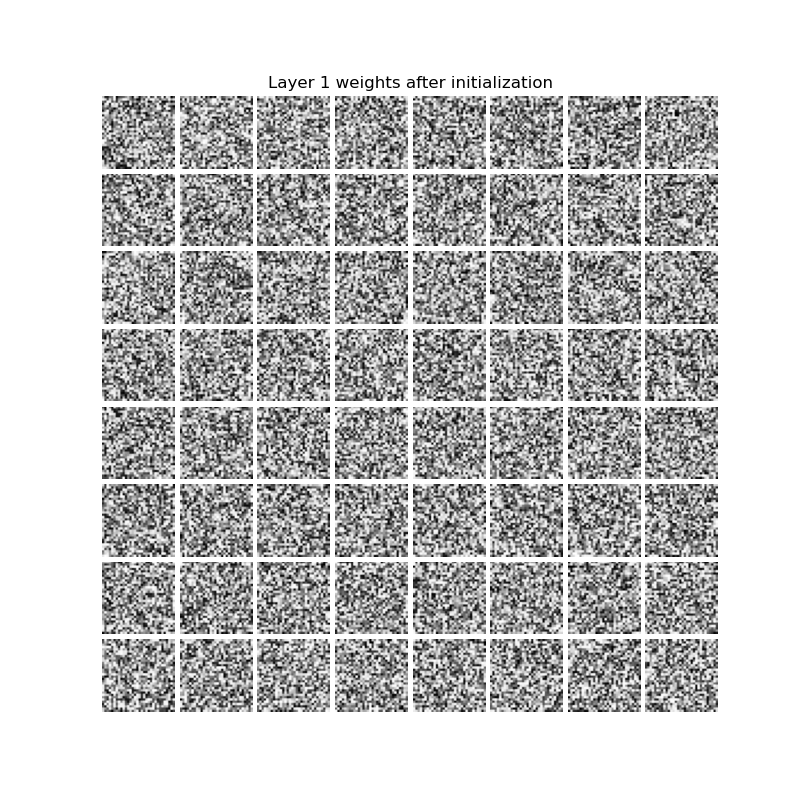
\includegraphics[width=0.45\textwidth]{figures/q_3_3_layer1_initial.png}  &  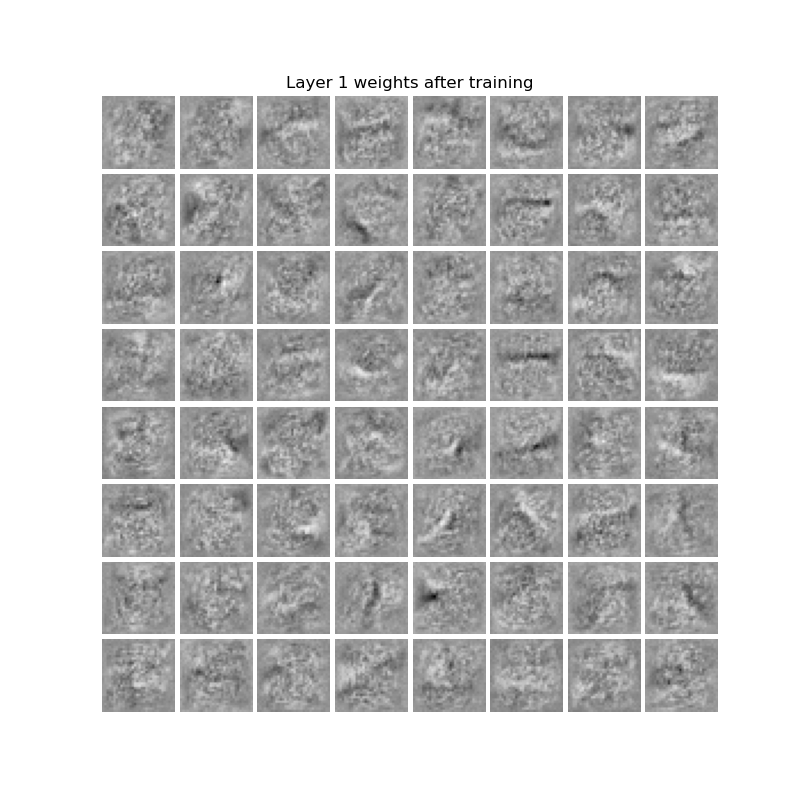
\includegraphics[width=0.45\textwidth]{figures/q_3_3_layer1_after_train.png}  \\  
    \textbf{(a)} After initialization but before training & \textbf{(b)} After training\\ [6pt] 
    \end{tabular}
    \caption{First layer weights after initialization but before training (a) and after training (b)}\label{fig:q_3_3}
\end{figure} 

\clearpage

\question{Q.3.4}{Visualize and include the confusion matrix of the test data for your best model. Comment on the top few pairs of classes that are most commonly confused.}

Figure \ref{fig:q_3_4} shows the confusion matrix of the test data for the best model trained. Notice the there few spots off the diagonal that are not zero (i.e. not dark blue), which indicates
the most misclassified pairs. In particular, the most commonly confused pairs observed were: (O, 0), (5, S) and (2, Z). This makes sense, as these
characters do look alike and depending on the handwriting even humans sometimes misrecongnize them.
\begin{figure}[h!]
    \centering   
    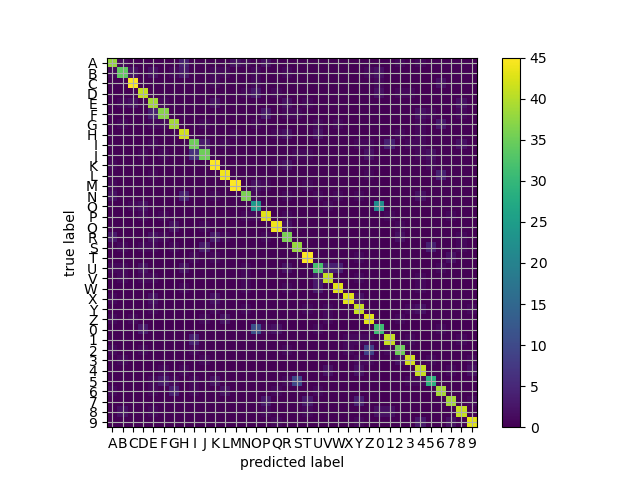
\includegraphics[width=0.75\textwidth]{figures/q_3_4_confusion_matrix.png}   \\       
    \caption{Confusion matrix of the test data}\label{fig:q_3_4}
\end{figure} 

\clearpage

\question{Q4.1}{The method outlined above is pretty simplistic, and while it
works for the given text samples, it makes several assumptions. What are two big assumptions that the sample method makes? In your writeup, include two example images where
you expect the character detection to fail (for example, miss valid letters, misclassify letters
or respond to non-letters).}
The extracting text method described in the handout makes the following assumptions:
\begin{itemize}
    \item characters from the same line are aligned horizontally
    \item there is enough white space between characters (both vertically and horizontally)
    \item characters in the same row have similar size
    \item characters are similar to the ones in the training dataset
\end{itemize}

Figures \ref{fig:q_4_1}(a)-(b) show examples where I expect the character detection algorithm to fail.

\begin{figure}[h!]
    \centering   
    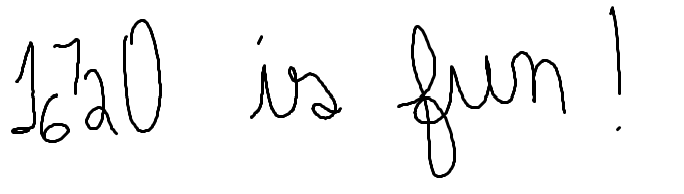
\includegraphics[width=0.5\textwidth]{figures/example_fail1.png}   \\  
    \textbf{(a)} Example 1 \\ [6pt] 
    
\includegraphics[width=0.5\textwidth]{figures/example_fail2.png}   \\  
    \textbf{(a)} Example 2 \\ [6pt] 

    \caption{Example images where character detection algorithm is expected to fail}\label{fig:q_4_1}
\end{figure} 

\clearpage
\question{Q4.2}{In n python/q4.py, implement the function findLetters. Include your code in the writeup.}

Figure \ref{fig:findletters} shows the code snippet of the function findLetters.
\begin{figure}[h!]
    \centering
    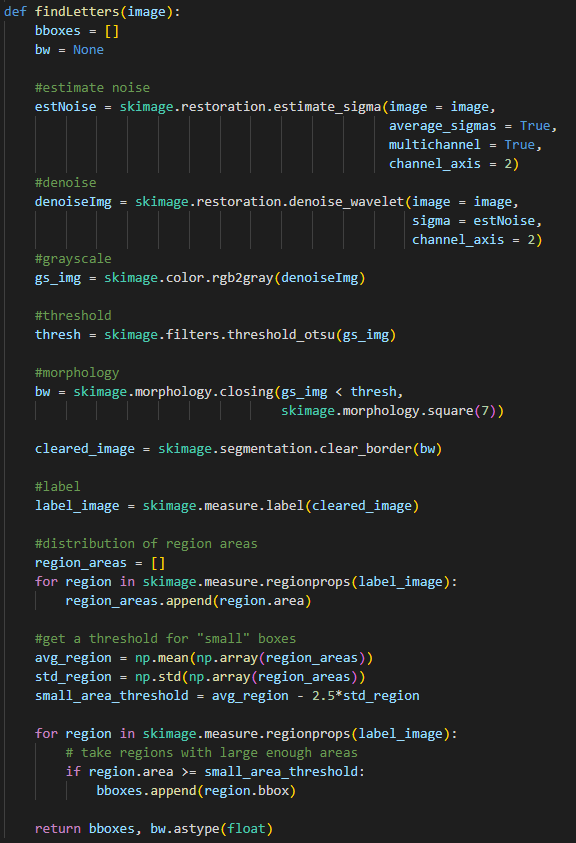
\includegraphics[width=0.65\textwidth]{figures/findletters_snapshot.png}
    \caption{Code snippet of the function findLetters.}
    \label{fig:findletters}
\end{figure}

\clearpage

\question{Q4.3}{Using python/run\_q4.py, visualize all of the located boxes on top of the binary image to show the accuracy of your findLetters function. 
Include all the resulting images in your writeup.}

Figures \ref{fig:q_4_23}(a)-(d) show the located bounding boxes for all sample images. All characters were captured properly, except the periods in the figure 01\_list.jpg.
\begin{figure}[h!]
    \centering
    \begin{tabular}{cccc}
    
    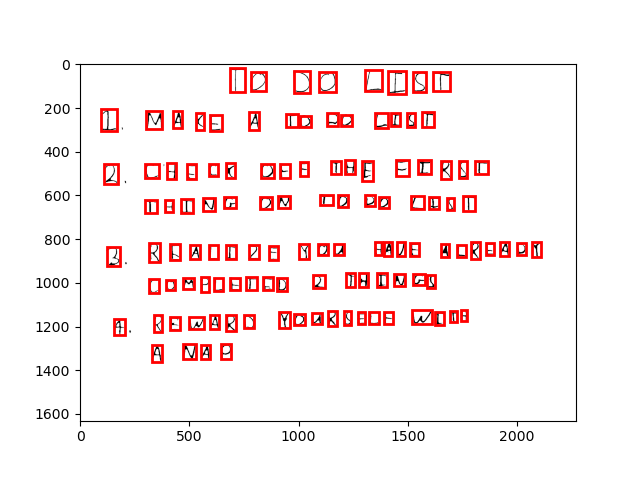
\includegraphics[width=0.45\textwidth]{figures/q_4_3_img_01_list.png}  &  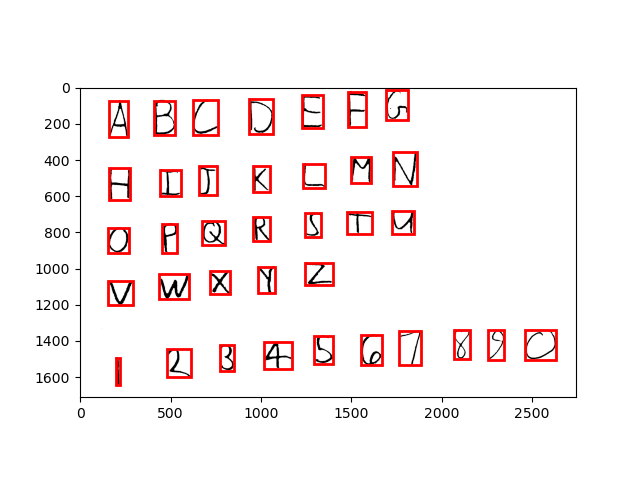
\includegraphics[width=0.45\textwidth]{figures/q_4_3_img_02_letters.png}  \\  
    \textbf{(a)} Image 01\_list.jpg & \textbf{(b)} Image 02\_letters.jpg\\ [6pt] 

    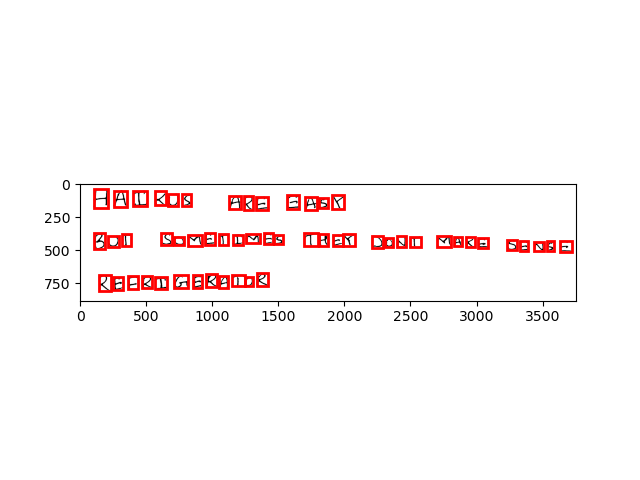
\includegraphics[width=0.45\textwidth]{figures/q_4_3_img_03_haiku.png}  &  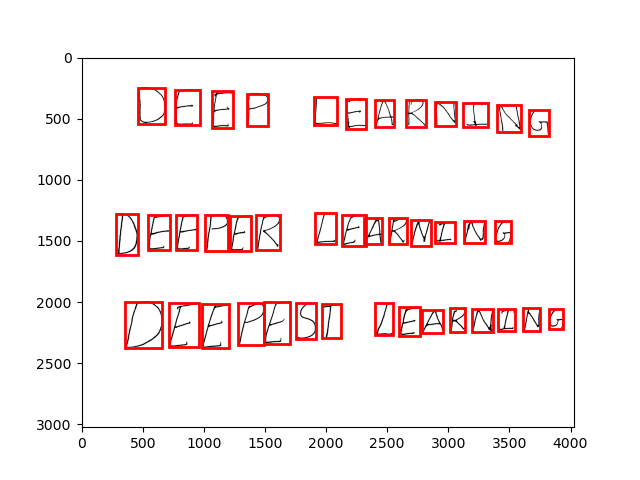
\includegraphics[width=0.45\textwidth]{figures/q_4_3_img_04_deep.png}  \\  
    \textbf{(c)} Image 03\_haiku.jpg & \textbf{(d)} Image 04\_deep.jpg\\ [6pt] 
    \end{tabular}
    \caption{Bounding boxes using function findLetters}\label{fig:q_4_23}
\end{figure} 


\clearpage

\question{Q.4}{Run your run\_q4.py on all of the provided sample images in images/. Include the extracted
text in your writeup. It is fine if your code ignores spaces, but if so, please add them manually
in the writeup.}

Table \ref{tbl:q_4_4} shows the characters extracted for each sample image. All had accuracy greater than 80\%.


\begin{table}[h!]
    \centering
    \caption{Character extracting results}\label{tbl:q_4_4}
    \begin{tabular}{ | c | c |c | }
      \hline
      Image & Text Extracted & Accuracy \\ \hline
      \begin{minipage}{.3\textwidth}
        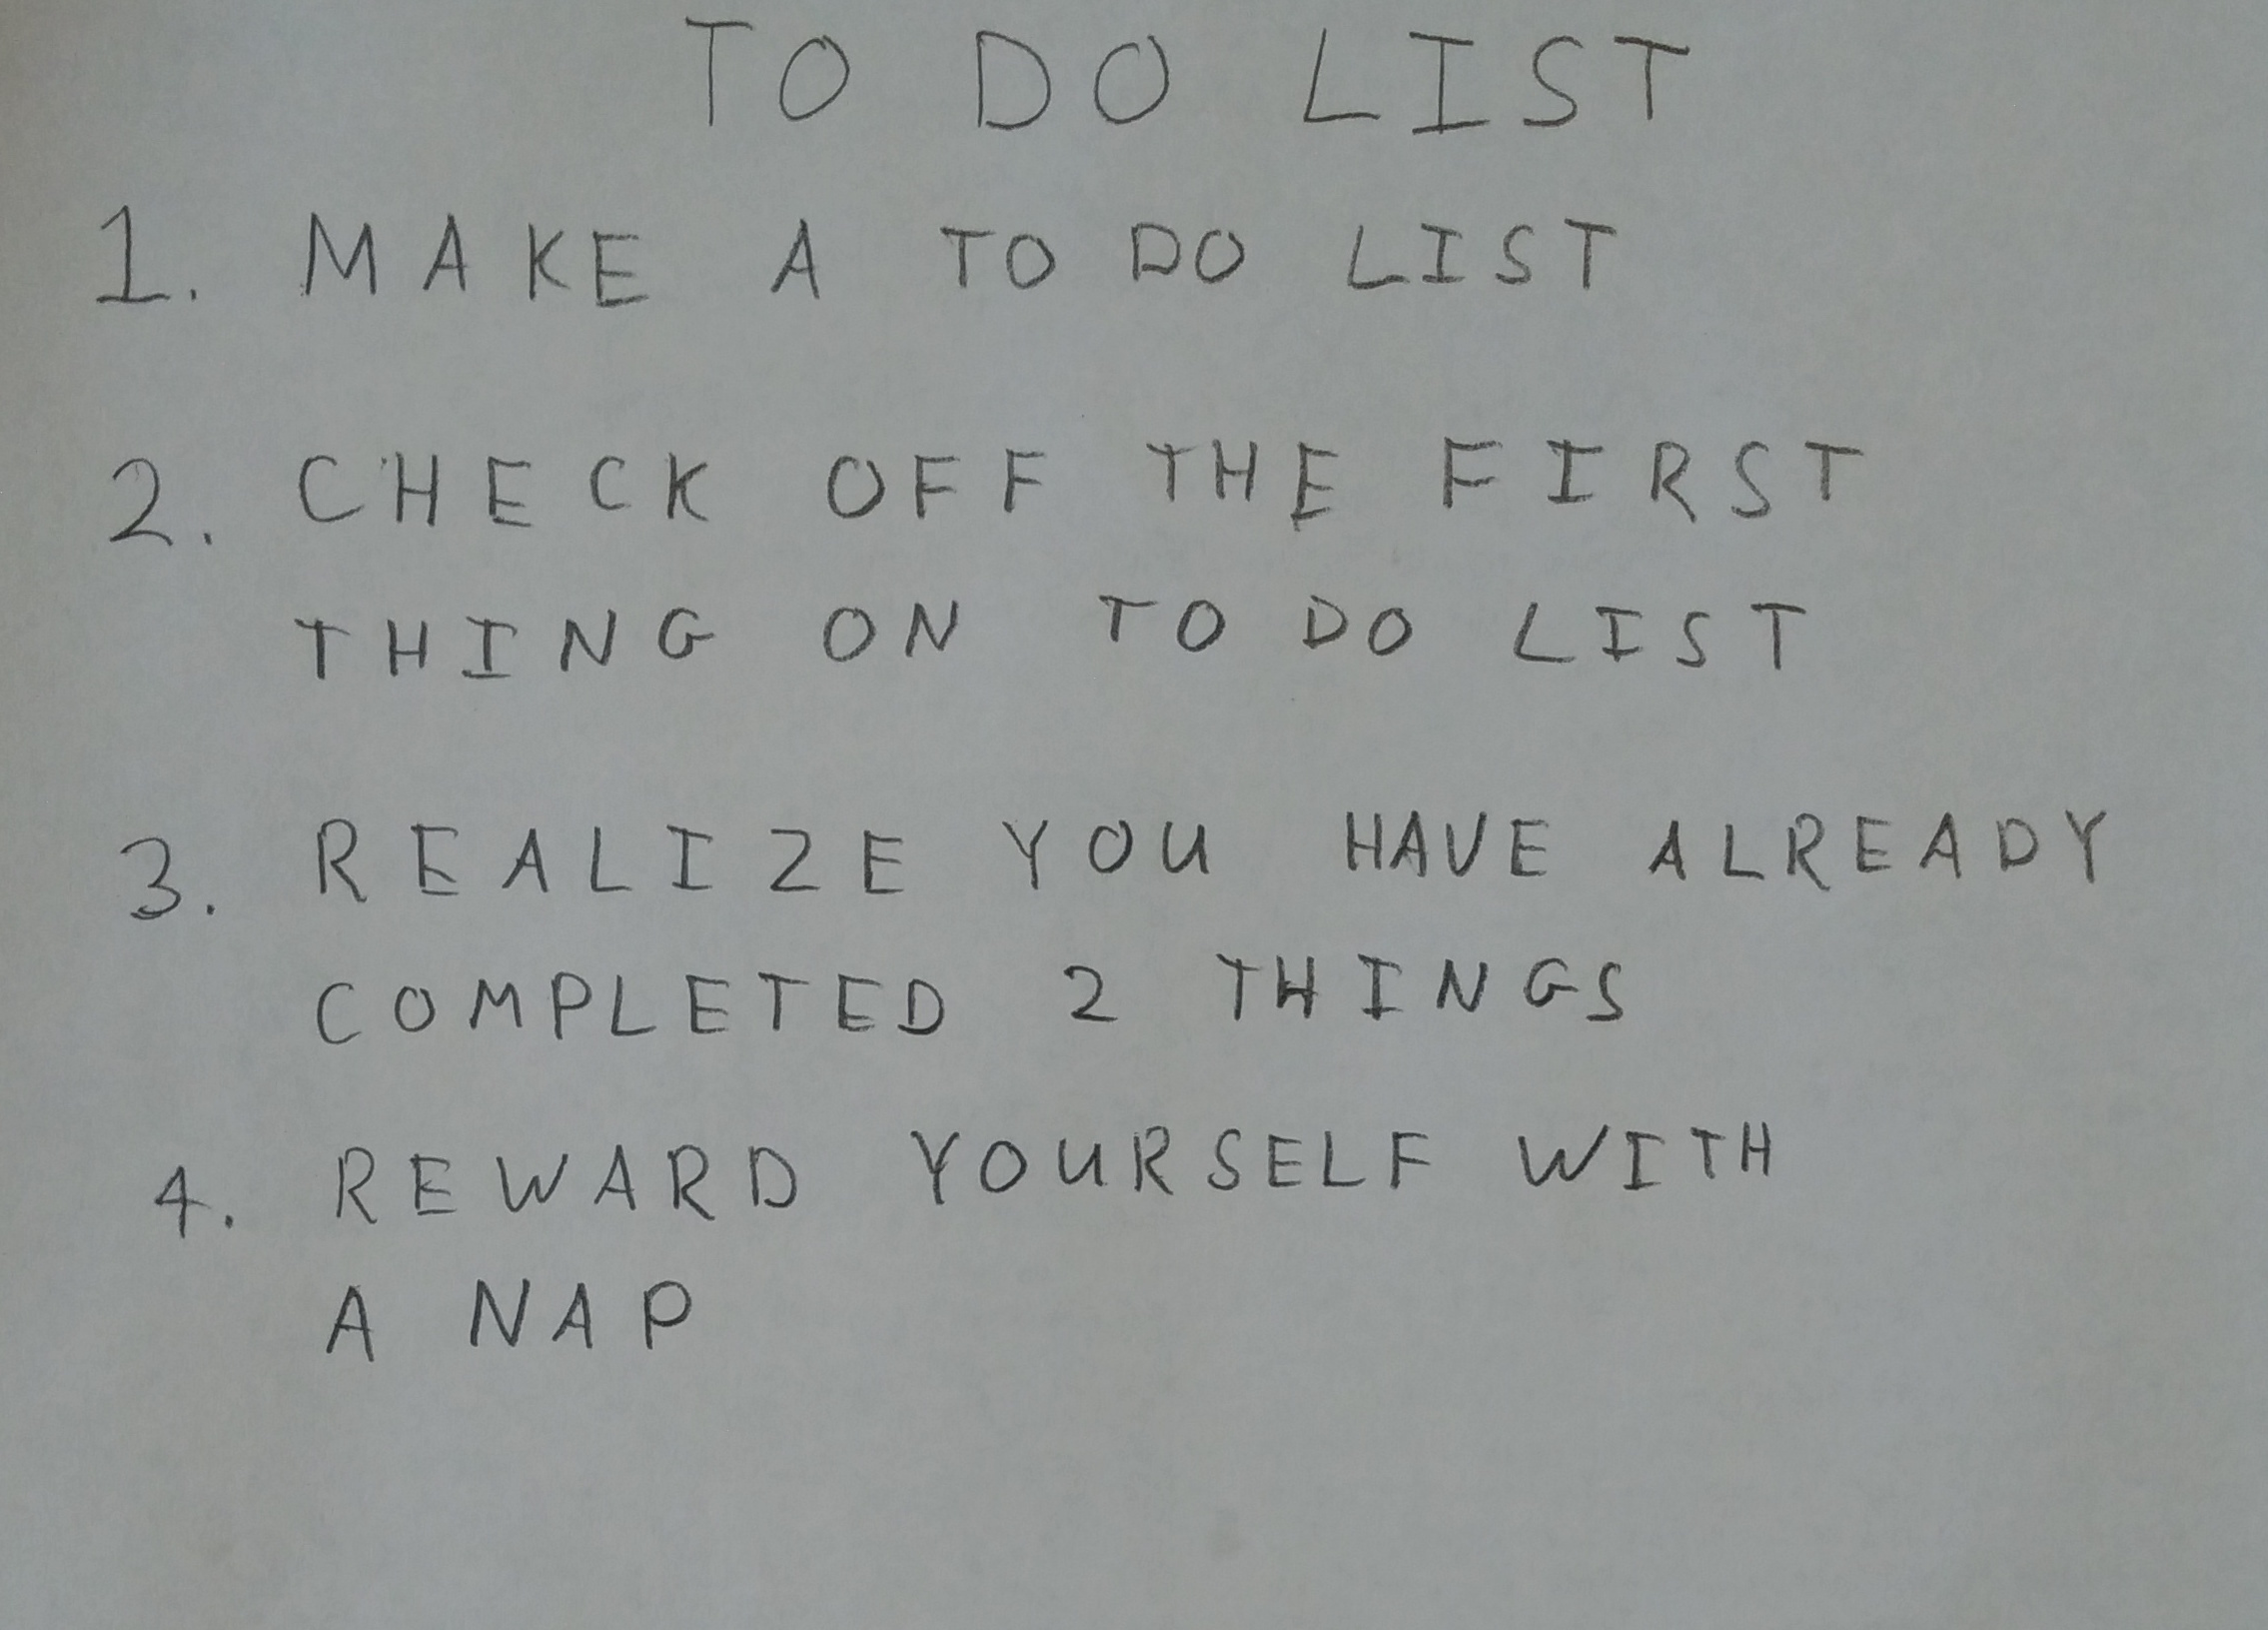
\includegraphics[width=0.85\textwidth]{figures/01_list.jpg}
      \end{minipage}
      &
      \makecell{T0 D0 LIST \\I HAKE A TO DO 6ZST\\2 CHKCK OFF YHE FZRST\\TH2HE OH TO DO L8ST\\3 RKALZZE YOU HAVE ALREADY\\COMPLETDD Z YHINOS\\4 REWARD YOURSELF WIYH\\A NAP} 
      & 
      81.7\%
      \\  \hline
      \begin{minipage}{.3\textwidth}
        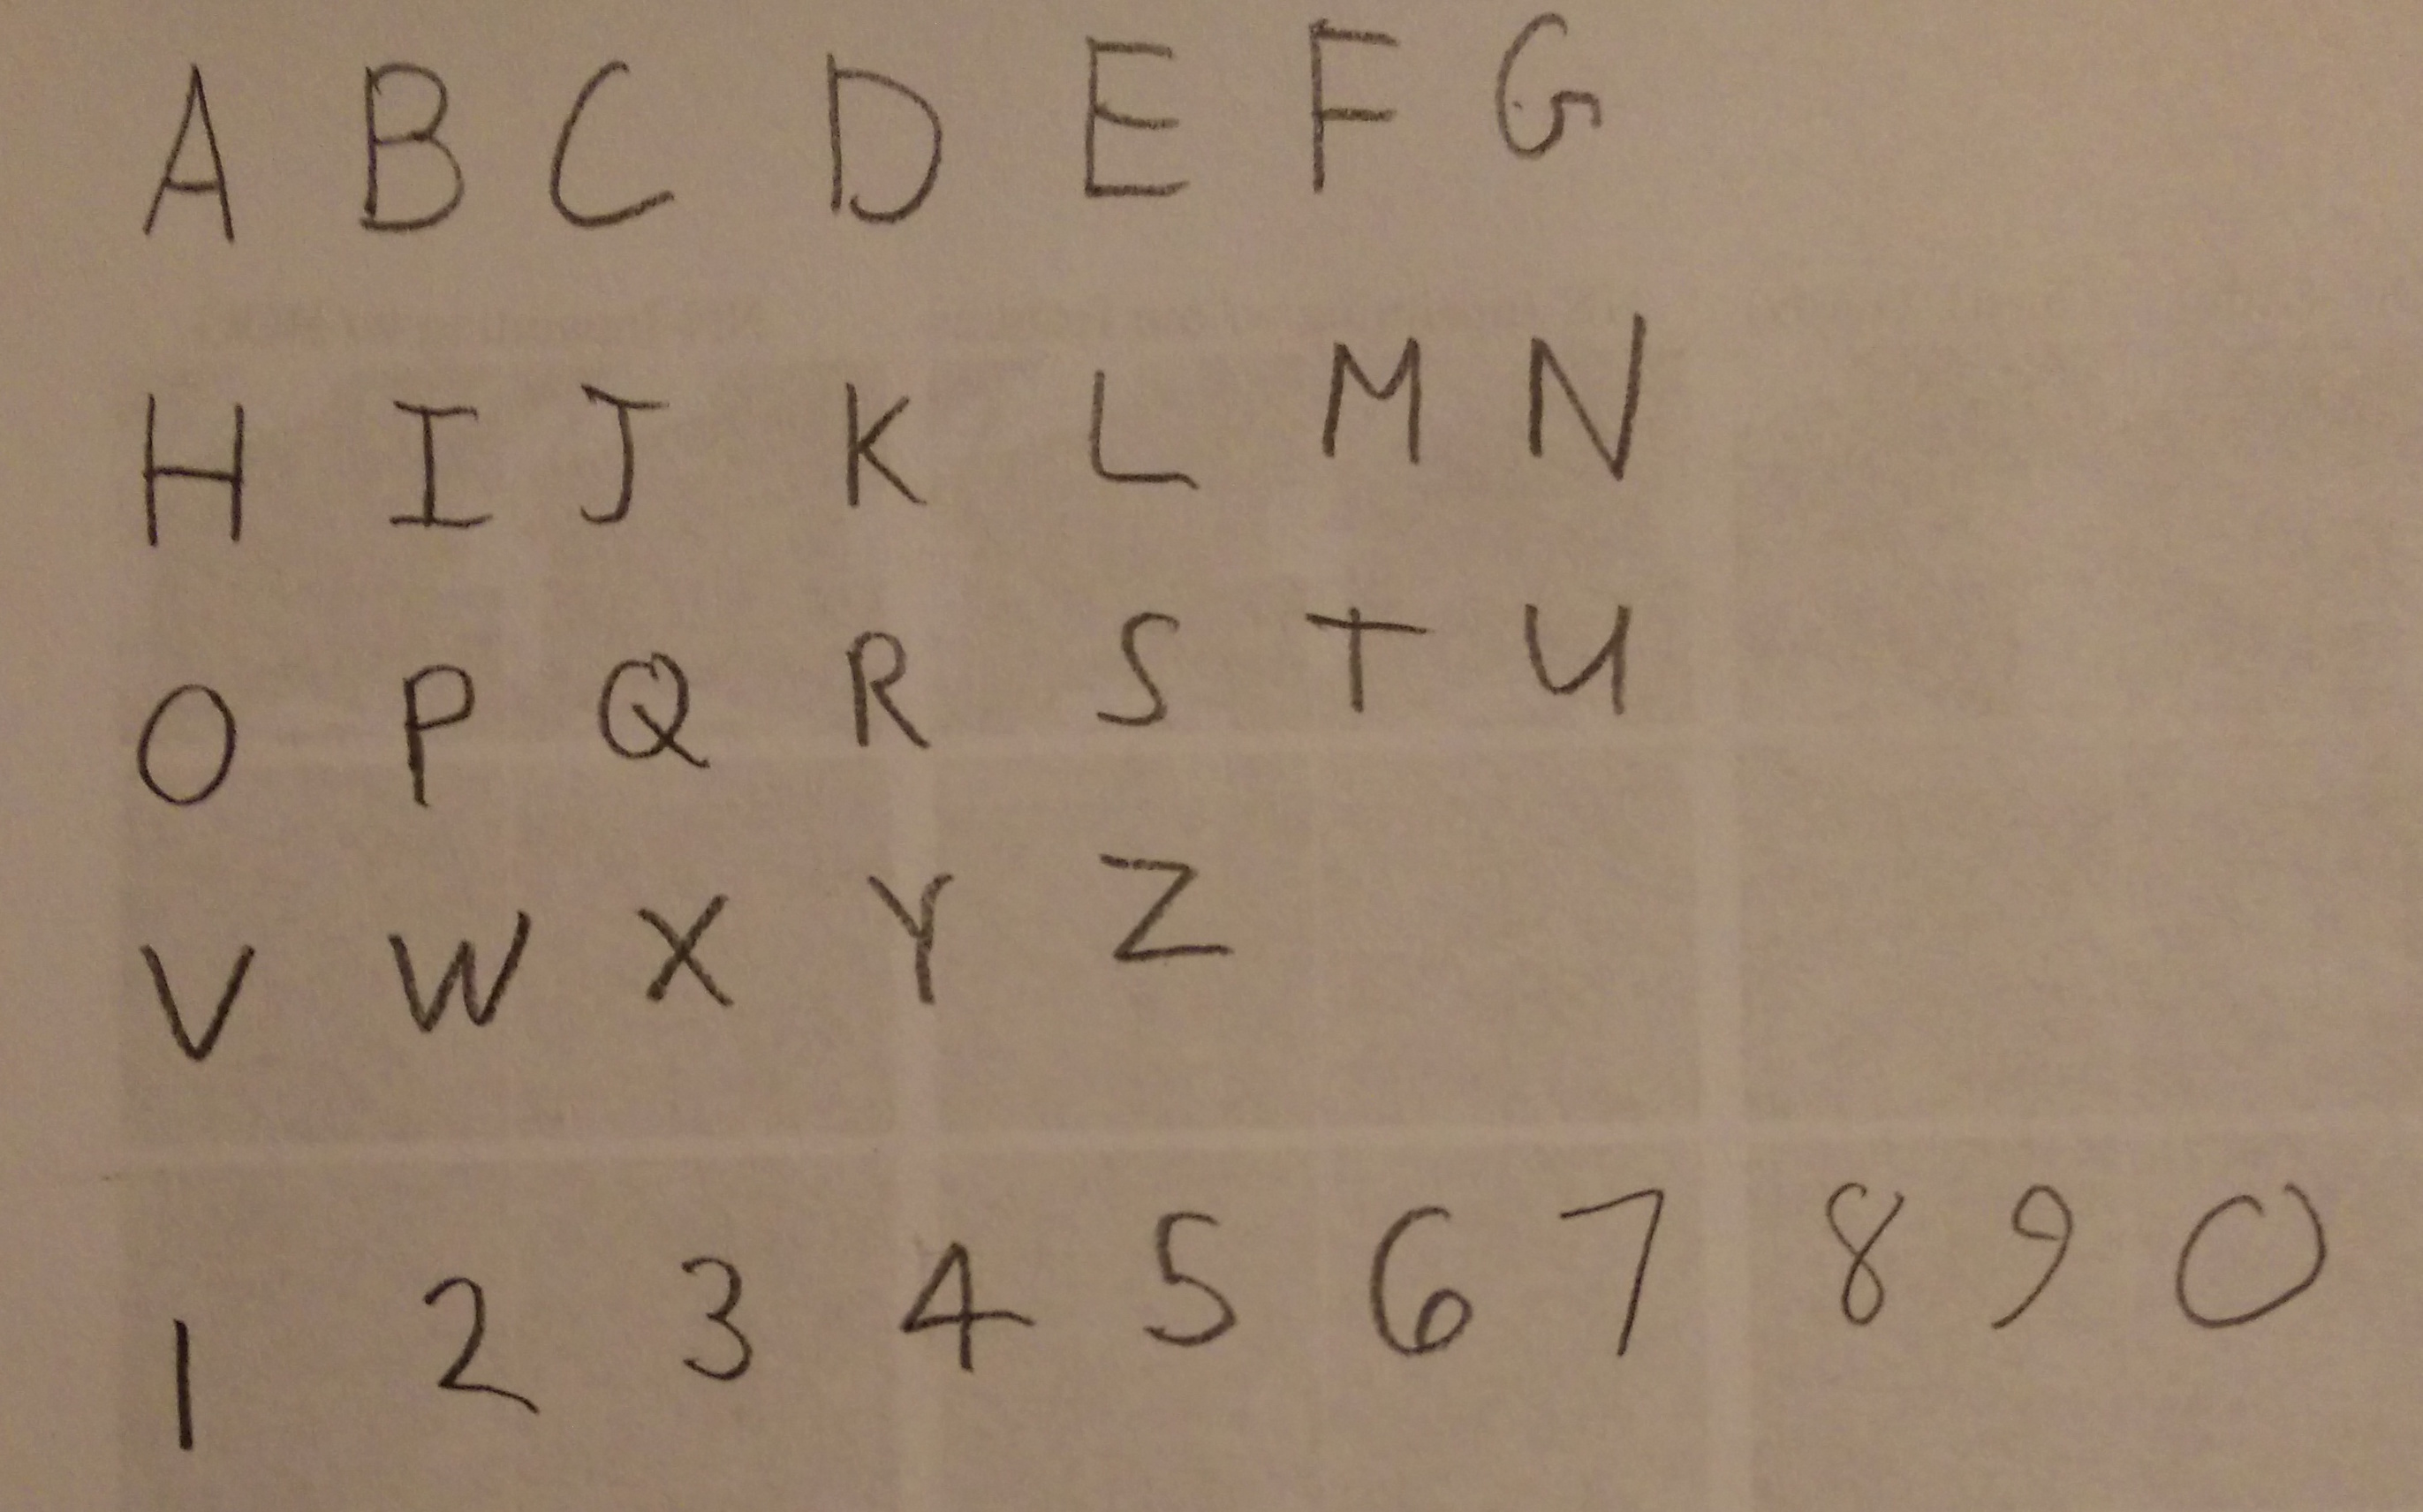
\includegraphics[width=0.85\textwidth]{figures/02_letters.jpg}
      \end{minipage}
      &
      \makecell{A B C D E F G\\H I J K L M N\\0 P Q R S T W\\V W X Y Z\\3 Z 3 Q 5 G 7 8 9 O} 
      & 
      80.6\% \\ \hline
      \begin{minipage}{.3\textwidth}
        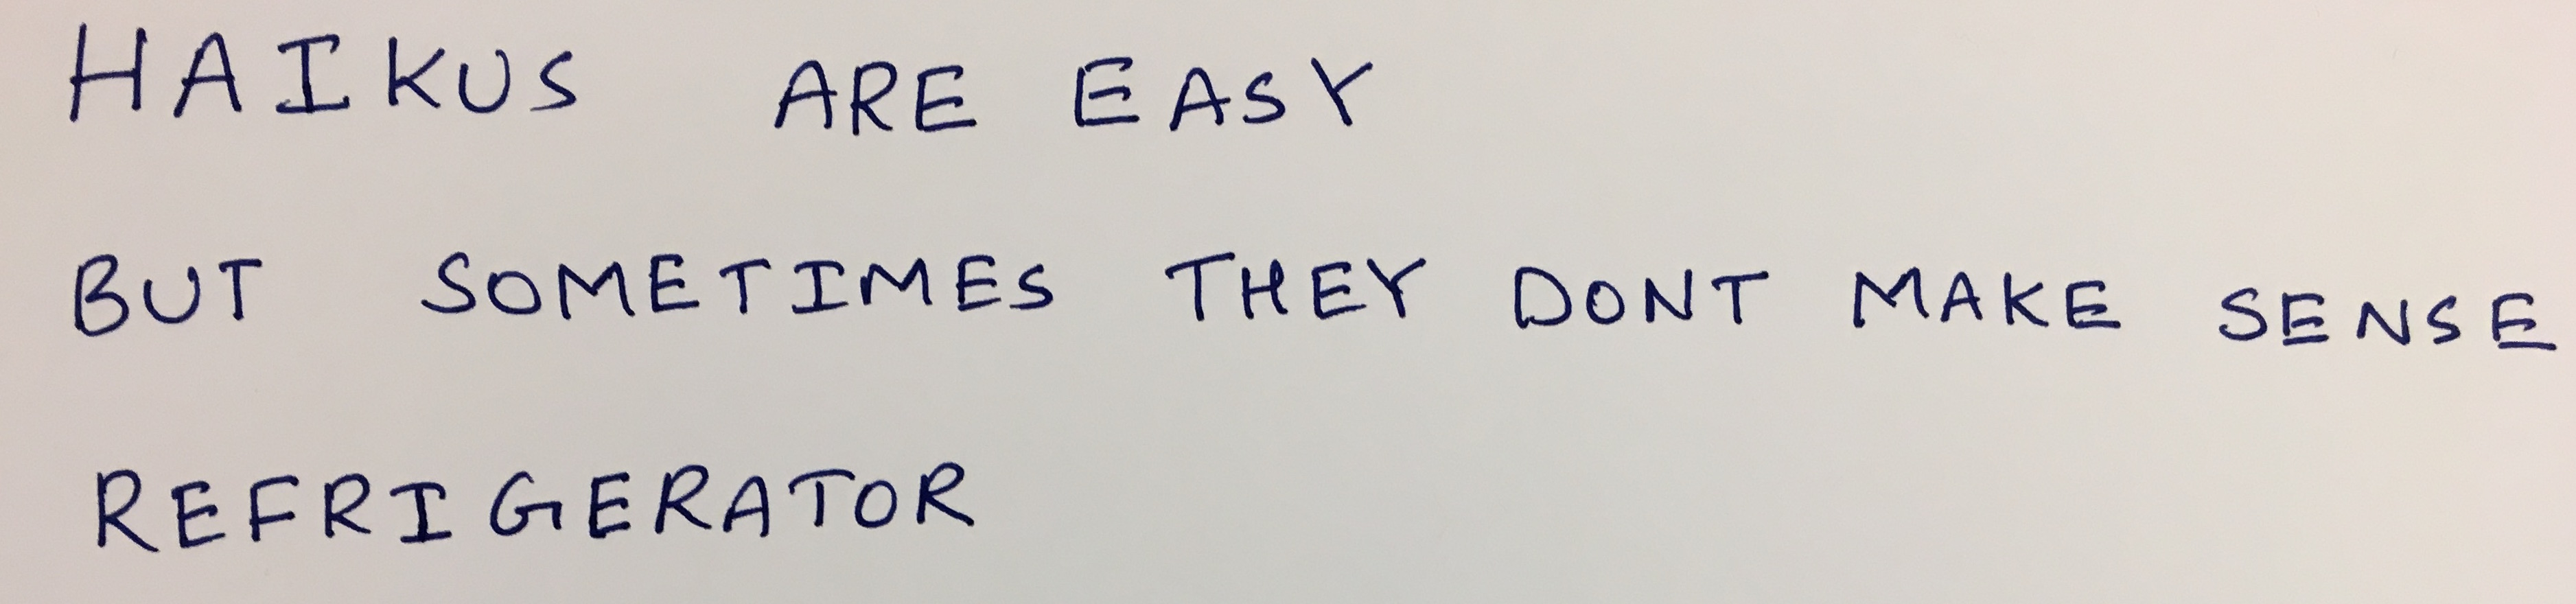
\includegraphics[width=0.85\textwidth]{figures/03_haiku.jpg}
      \end{minipage}
      &
      \makecell{HAIKUS ARE EASY\\BUT SOMETIMES TREY D0NT MAKE SEMSE\\REFRIGERAT0R} 
      & 
      92.6\% \\ \hline
      \begin{minipage}{.3\textwidth}
        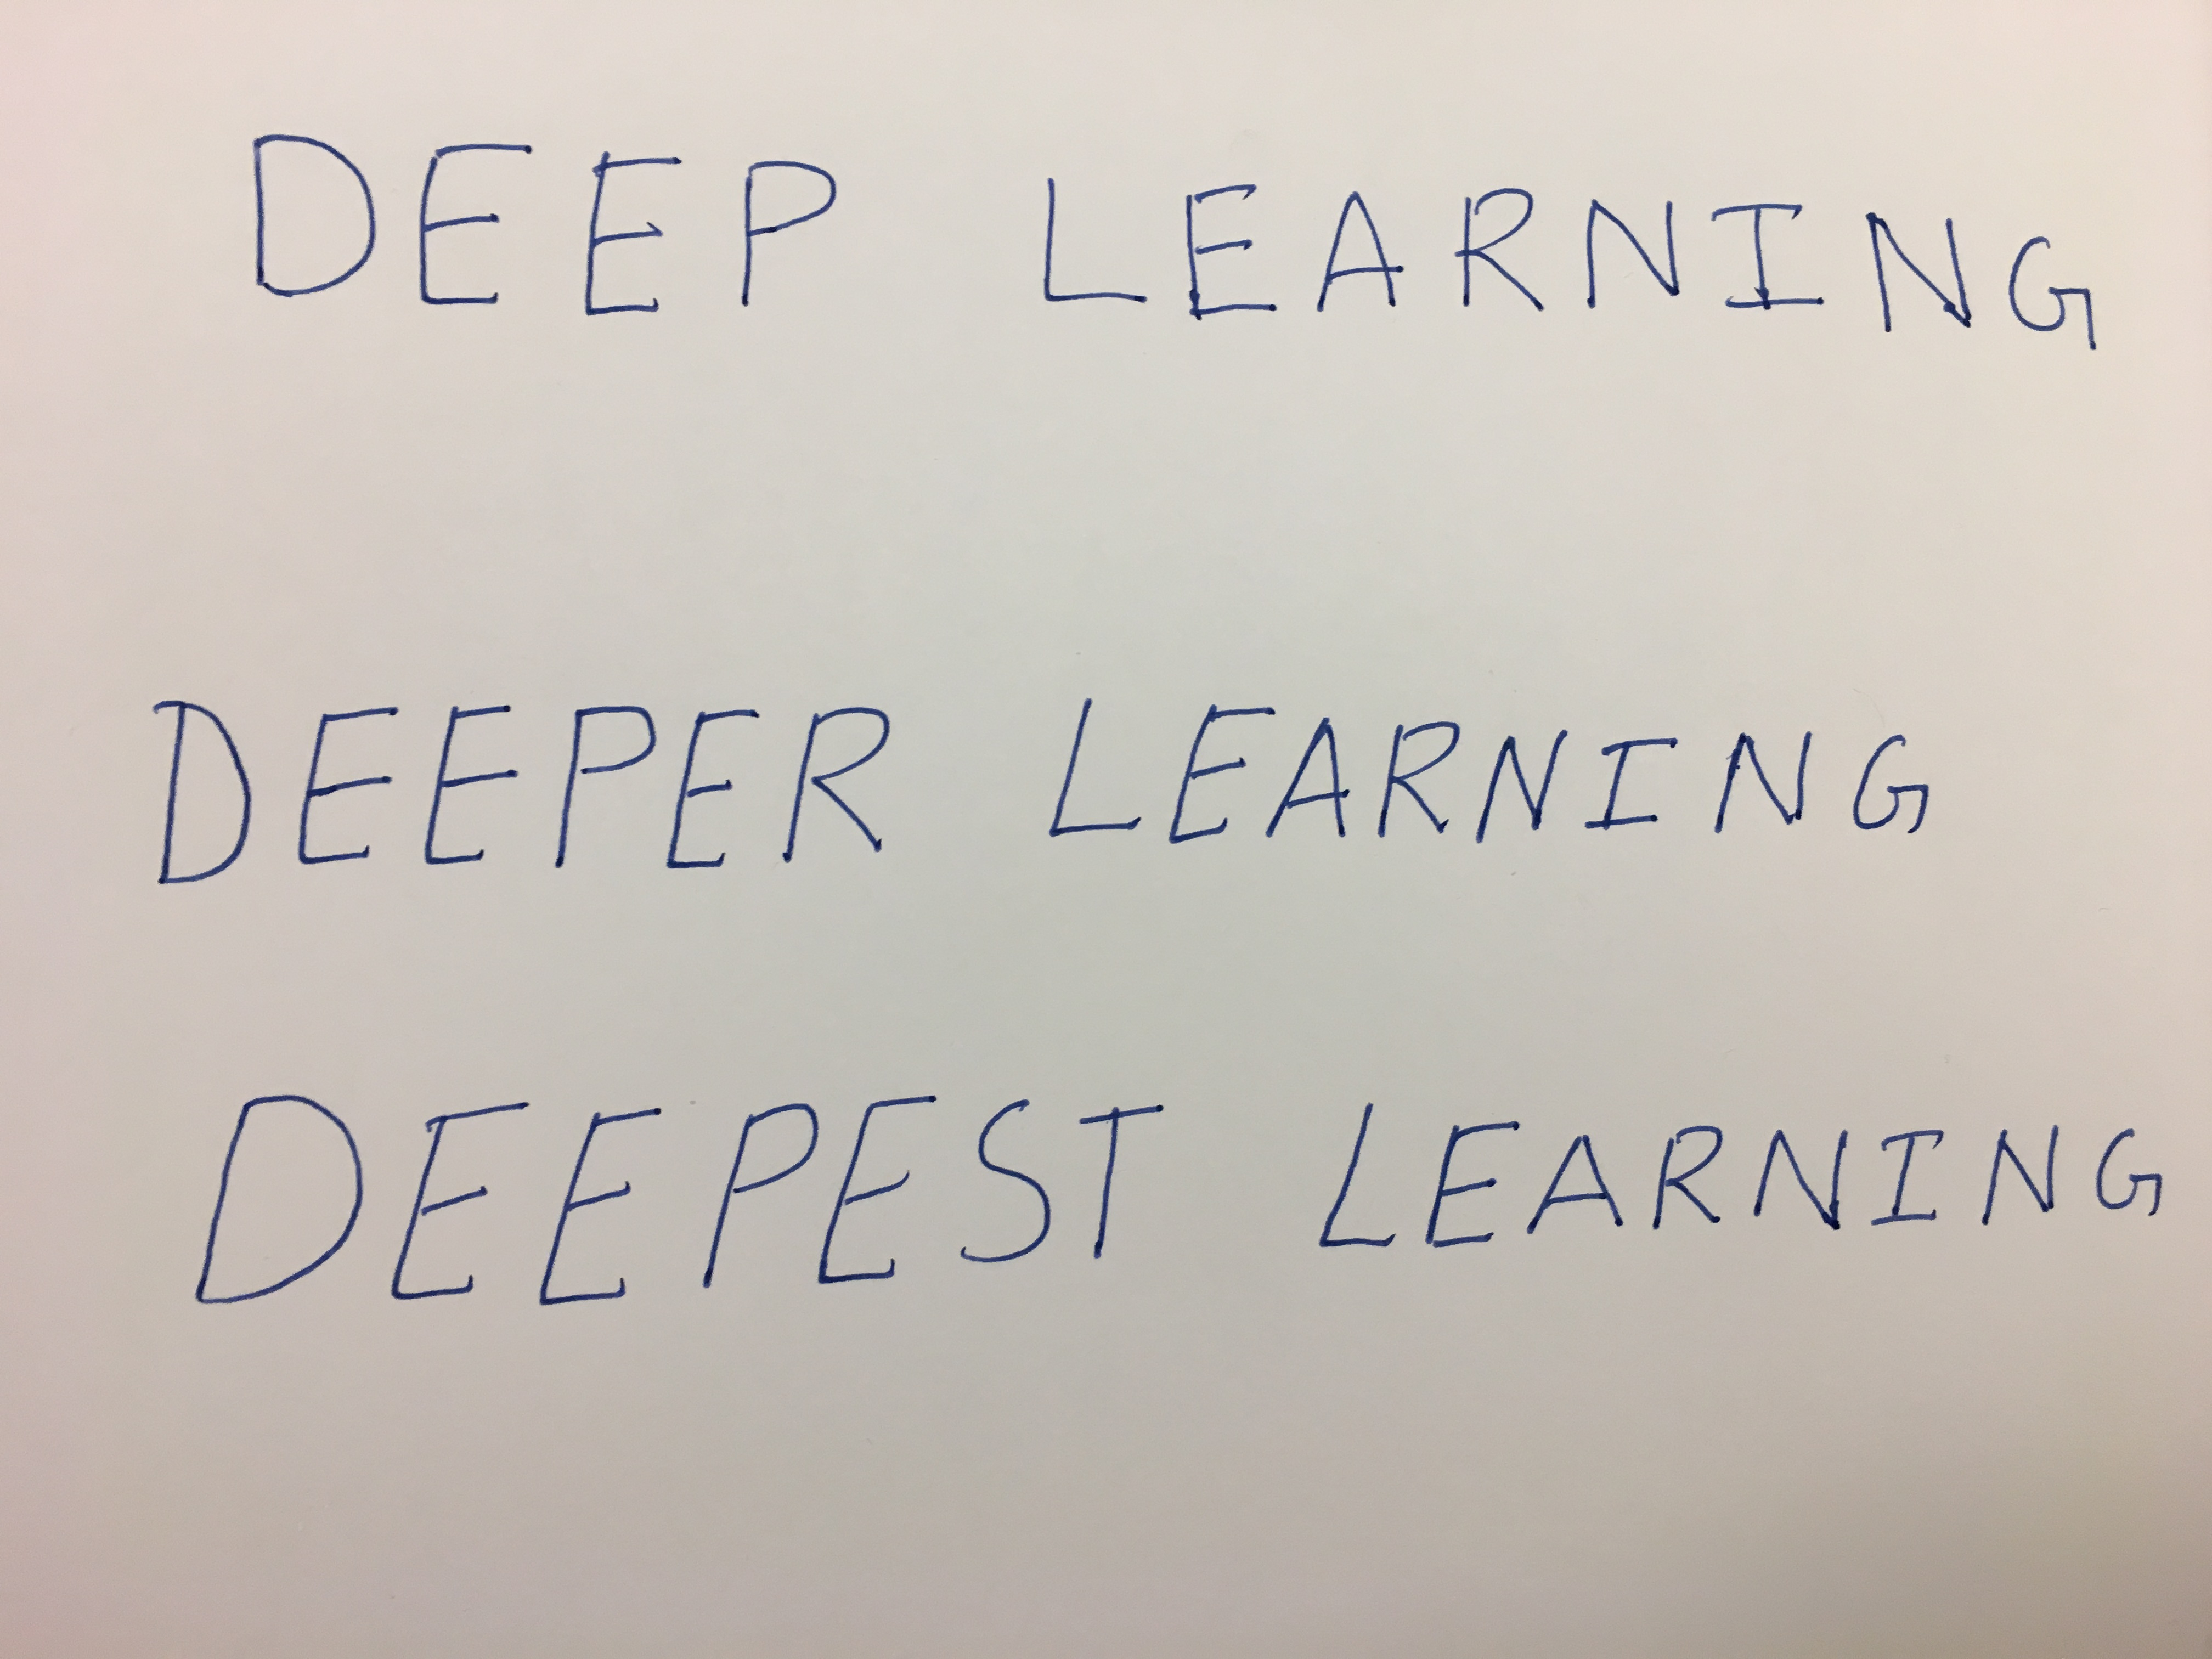
\includegraphics[width=0.85\textwidth]{figures/04_deep.jpg}
      \end{minipage}
      &
      \makecell{DEEF LEARMING\\DHHPER LEARHING\\DFEFFST LEARNING} 
      & 
      80.5\% \\ \hline      

    \end{tabular}       
  \end{table}

\clearpage

\question{Q5.1.1}{Implement the autoencoder specified in the handout. Include your code in the writeup.}

Figure \ref{fig:auto_encoder} shows the code snippet of the autoencoder specified in the handout.
\begin{figure}[h!]
    \centering
    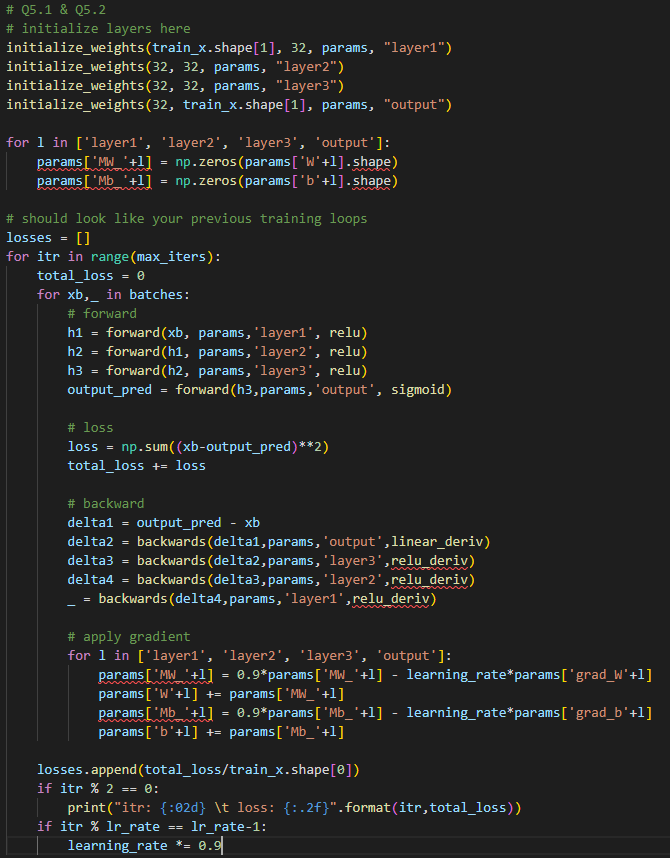
\includegraphics[width=0.65\textwidth]{figures/auto_encoder_snapshot.png}
    \caption{Code snippet of the autoencoder specified in the handout.}
    \label{fig:auto_encoder}
\end{figure}


\clearpage

\question{Q5.1.2}{Implement momentum. Include your code in the writeup.}

Figure \ref{fig:auto_encoder2} shows the code snippet of the autoencoder (with momentum) specified in the handout.
\begin{figure}[h!]
    \centering
    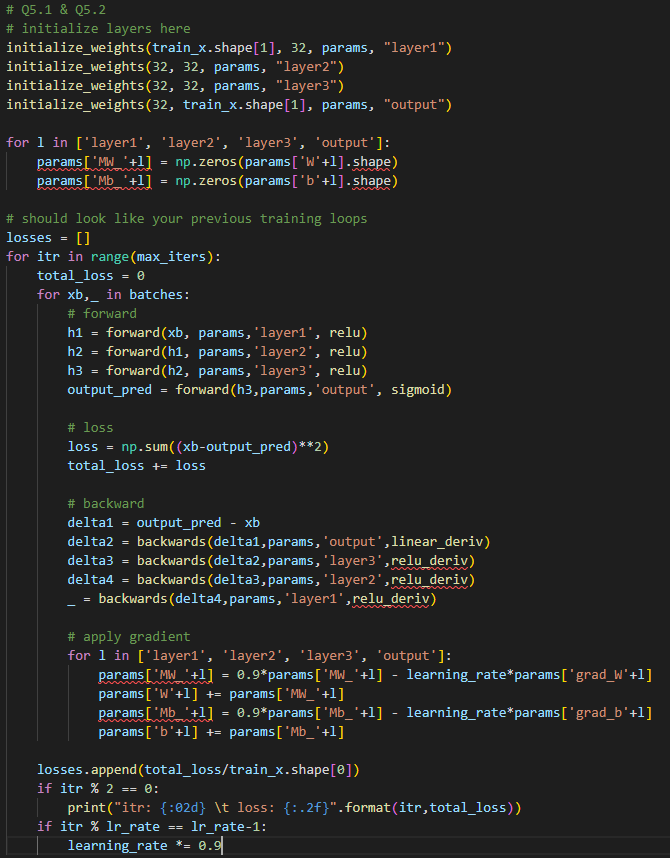
\includegraphics[width=0.65\textwidth]{figures/auto_encoder_snapshot.png}
    \caption{Code snippet of the autoencoder (with momentum) specified in the handout.}
    \label{fig:auto_encoder2}
\end{figure}

\clearpage

\question{Q5.2}{Using the provided default settings, train the network for 100 epochs. Plot the training loss curve and include it in the writeup.
What do you observe?}


Figure \ref{fig:q_5_2} shows the encoder training loss curve. The averge loss drops fairly quickly in the first 5 epochs and then gradually declines afterwards.

\begin{figure}[h!]
    \centering   
    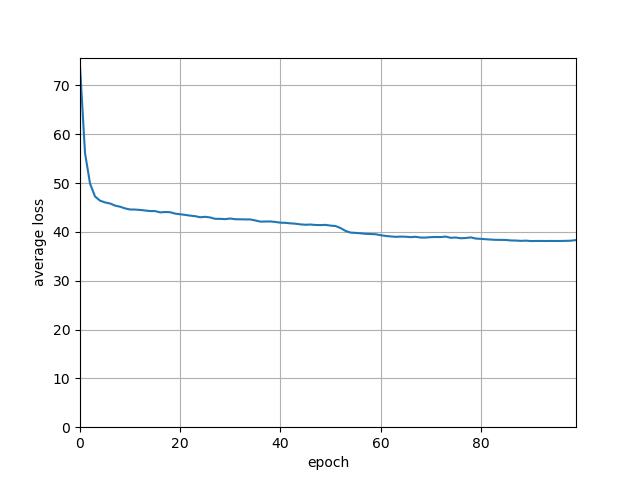
\includegraphics[width=0.65\textwidth]{figures/q_5_2_loss.png}   \\       
    \caption{Training loss curve}\label{fig:q_5_2}
\end{figure} 

\clearpage

\question{5.3.1}{Select 5 classes from the total 36 classes in the validation set and for each selected class include in your report 2 validation images and their reconstruction.
What differences do you observe in the reconstructed validation images compared to the original ones?}

Figure \ref{fig:q_5_3_1} shows 10 validations images (2 for each class) for the classes A, B, C, 1 and 2. The columns 1 and 3 represent the original images, while columns 2 and 4 
are the corresponding reconstructed versions. The reconstructed versions are blurry, and also seems to misrepresent some characters (e.g. reconstruction version of 2 looks like a Z).

\begin{figure}[h!]
    \centering   
    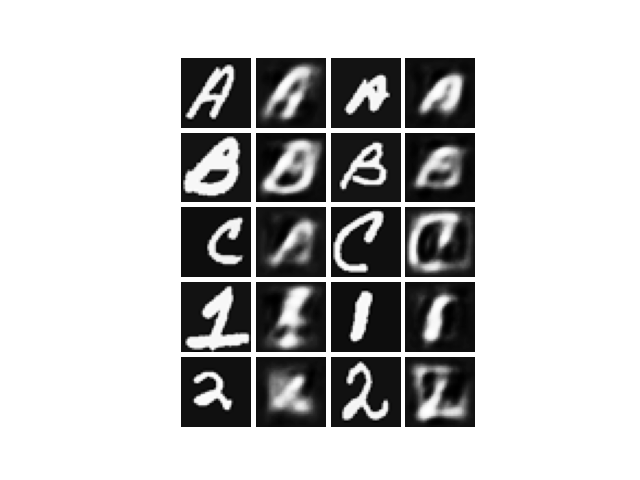
\includegraphics[width=0.65\textwidth]{figures/q_5_3_1_comparison.png}   \\       
    \caption{Auto encoder - Original (columns 1 and 3) versus reconstructed (columns 2 and 4) images}\label{fig:q_5_3_1}
\end{figure} 


\clearpage

\question{Q5.3.2}{ Report the average PSNR you get from the autoencoder across all images in the validation set}
The average PSNR was 14.55.


\clearpage
\question{Q6.1.1}{Re-write and re-train your fully-connected network on the included NIST36 in PyTorch. Plot training accuracy and loss over time.}

Figures \ref{fig:q_6_1_1} (a)-(b) show respectively the loss and accuracy over the epochs using PyTorch, both for training and validation sets. 
\begin{figure}[h!]
    \centering
    \begin{tabular}{cccc}
    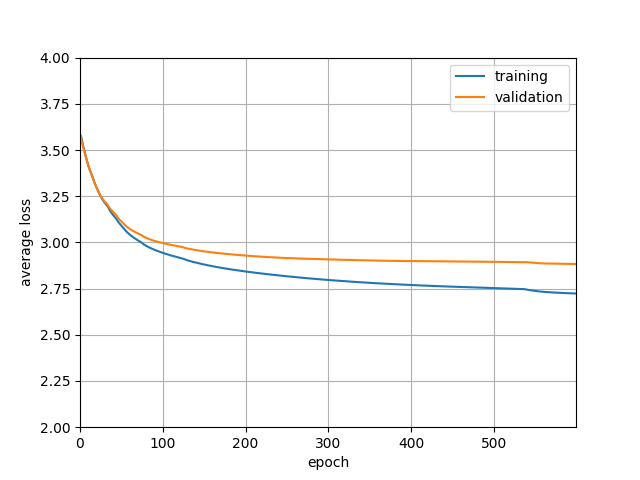
\includegraphics[width=0.45\textwidth]{figures/q_6_1_1_loss.png}  &  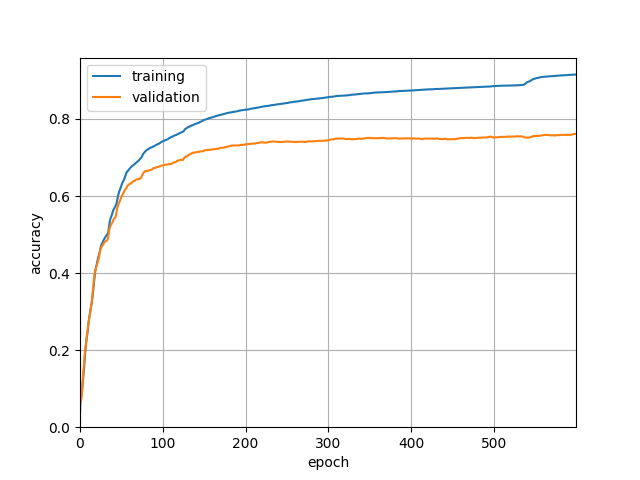
\includegraphics[width=0.45\textwidth]{figures/q_6_1_1_accuracy.png}  \\  
    \textbf{(a)} Loss by epoch step & \textbf{(b)} Accuracy by epoch step\\ [6pt] 
    \end{tabular}
    \caption{Loss and accuracy over the epochs for training (blue lines) and validation (orange lines) datasets - using PyTorch}\label{fig:q_6_1_1}
\end{figure} 


Figure \ref{fig:cnn1} shows the code snippet of the fully-connected network implemented using PyTorch.
\begin{figure}[h!]
    \centering
    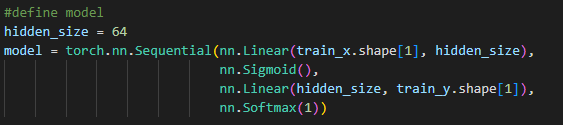
\includegraphics[width=0.55\textwidth]{figures/cnn_q611_snapshot.png}
    \caption{Code snippet of the fully-connected network implemented using PyTorch}
    \label{fig:cnn1}
\end{figure}

\clearpage

\question{Q6.1.2}{Train a convolutional neural network with PyTorch on the included NIST36 dataset. Compare its performance with the previous fully-connected
network.}
I implemented a convolutional neural network fairly similar to the Lenet model (see Figure \ref{fig:cnn2}). The validation accuracy of the fully-connected network was 77.4\% while for the CNN model
was 84.5\%. 

Figure \ref{fig:cnn2} shows the code snippet of the CNN implemented using PyTorch.
\begin{figure}[h!]
    \centering
    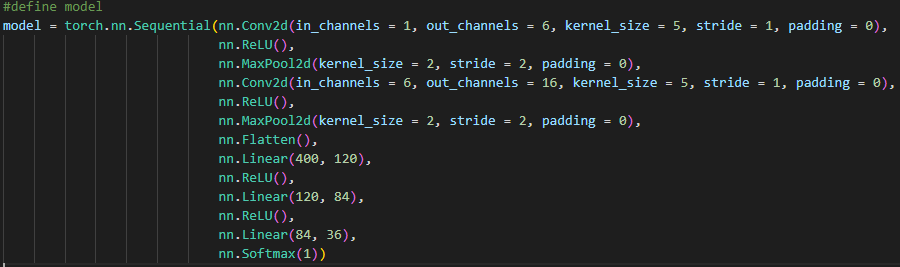
\includegraphics[width=0.65\textwidth]{figures/cnn_q612_snapshot.png}
    \caption{Code snippet of the CNN implemented using PyTorch - NIST36 dataset}
    \label{fig:cnn2}
\end{figure}

\clearpage

\question{Q6.1.3}{Train a convolutional neural network with PyTorch on CIFAR-10 (torchvision.datasets.CIFAR10). Plot training accuracy and loss over time.}
I implemented a convolutional neural network fairly similar to the Lenet model (see Figure \ref{fig:cnn3}). Figures \ref{fig:q_6_1_3} (a)-(b) show respectively the training loss and accuracy over the epochs for this model.
\begin{figure}[h!]
    \centering
    \begin{tabular}{cccc}
    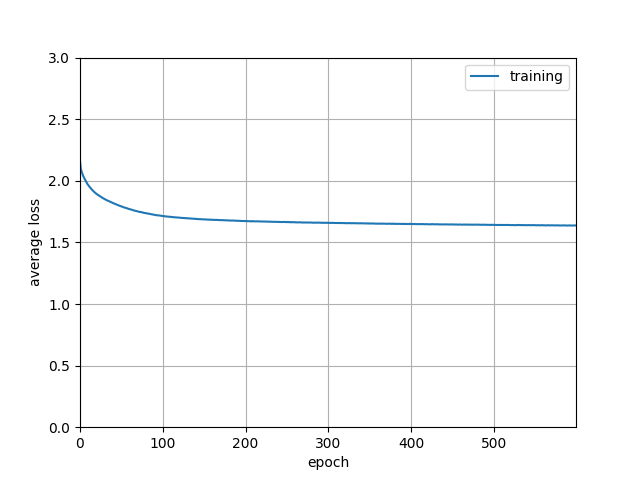
\includegraphics[width=0.45\textwidth]{figures/q_6_1_3_loss.png}  &  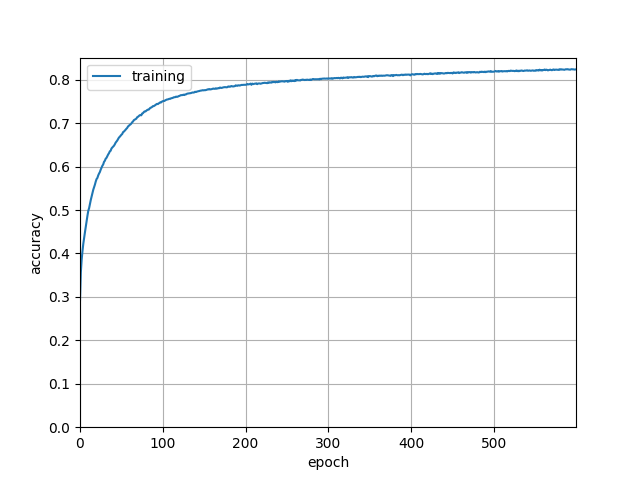
\includegraphics[width=0.45\textwidth]{figures/q_6_1_3_accuracy.png}  \\  
    \textbf{(a)} Loss by epoch step & \textbf{(b)} Accuracy by epoch step\\ [6pt] 
    \end{tabular}
    \caption{Training loss and accuracy over the epochs - CIFAR-10 dataset}\label{fig:q_6_1_3}
\end{figure} 

Figure \ref{fig:cnn3} shows the code snippet of the CNN implemented using PyTorch.
\begin{figure}[h!]
    \centering
    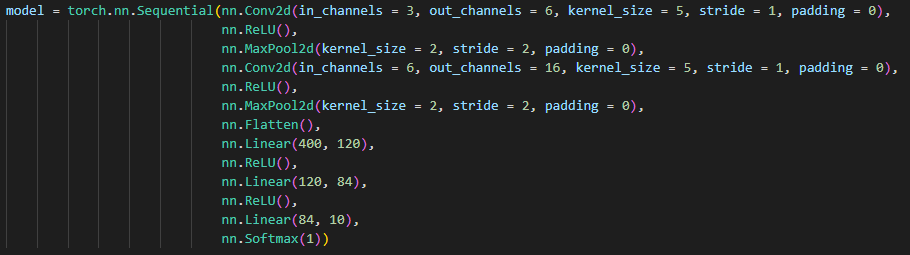
\includegraphics[width=0.65\textwidth]{figures/cnn_q613_snapshot.png}
    \caption{Code snippet of the CNN implemented using PyTorch - CIFAR-10 dataset}
    \label{fig:cnn3}
\end{figure}

\clearpage

\question{Q6.1.4}{Use the same dataset in HW1, and implement a convolutional neural network with PyTorch for scene classification.
Compare your result with the one you got in HW1, and briefly comment on it.}

Using a fairly similar LeNet model (see Figure \ref{fig:cnn4}), I obtained 45.6\% test accuracy.  In HW1, the best model I found had test accuracy of 62\%.  The CNN model tried here was a ``quick-and-dirt'' approach.
I believe it is possible to tweak the model (e.g. add more convolutional layers, use higher resolution) to improve test accuracy.

Figure \ref{fig:cnn4} shows the code snippet of the CNN implemented using PyTorch.
\begin{figure}[h!]
    \centering
    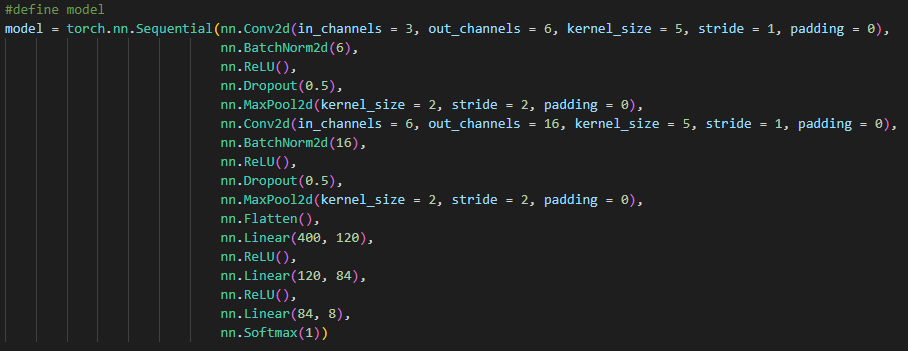
\includegraphics[width=0.65\textwidth]{figures/cnn_q614_snapshot.png}
    \caption{Code snippet of the CNN implemented using PyTorch - SUN dataset}
    \label{fig:cnn4}
\end{figure}

\clearpage

\question{Q6.2}{Fine tuning}
I skipped this question.

\clearpage

\question{Q6.3}{Neural networks in the RealWorld}
I downloaded the ResNet50 pretrained image classification model from torchvision, and the $64\times64$ ImageNet validation data.  I chose the category 'Rottweiler'.  There were 50 images in the validation set with images of rottweilers. Out of these 50, the Resnet50 model
predicted correctly 21 (42.0\%) of them. This model misclassified 23 (46.0\%) of the 'Rottweiler' images as 'Black-and-tan coonhound' images, which is understandable since both dog breeds have similar colors, and the image
resolution is low. When considering top-5 prediction, the ResNet50 accuracy of rottweiler images was 86.0\%.

I chose a video of a rotweiller in a cage, which had 270 frames in total and the rotweiller was present in every single frame. Figures \ref{fig:q_6_3} (a)-(d) shows four frames of the video.

\begin{figure}[h!]
    \centering
    \begin{tabular}{cccc}
    
    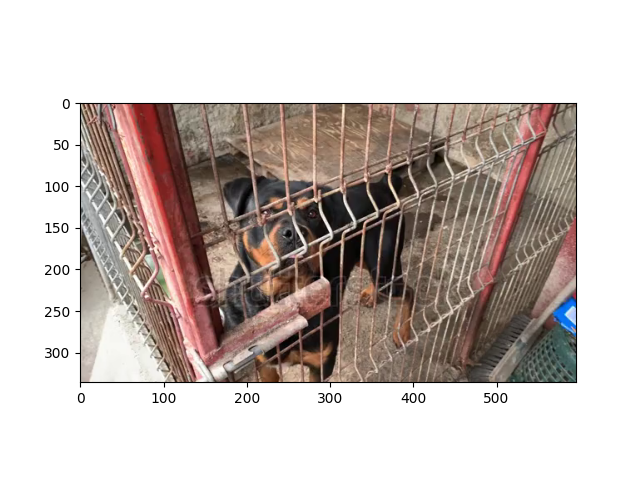
\includegraphics[width=0.45\textwidth]{figures/q_6_3_rot0.png}  &  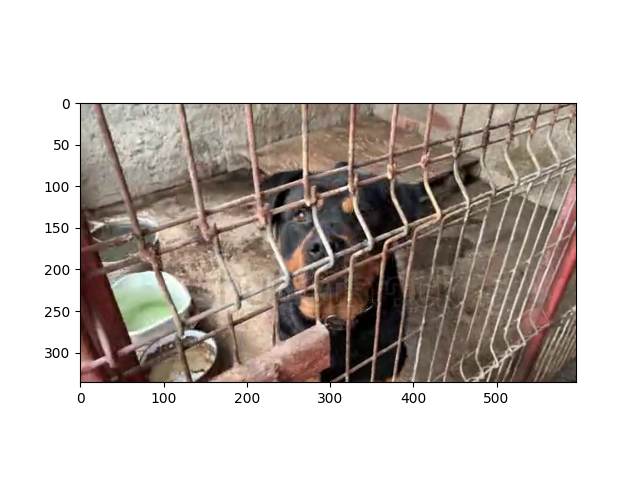
\includegraphics[width=0.45\textwidth]{figures/q_6_3_rot89.png}  \\  
    \textbf{(a)} Frame 0 & \textbf{(b)} Frame 90\\ [6pt] 

    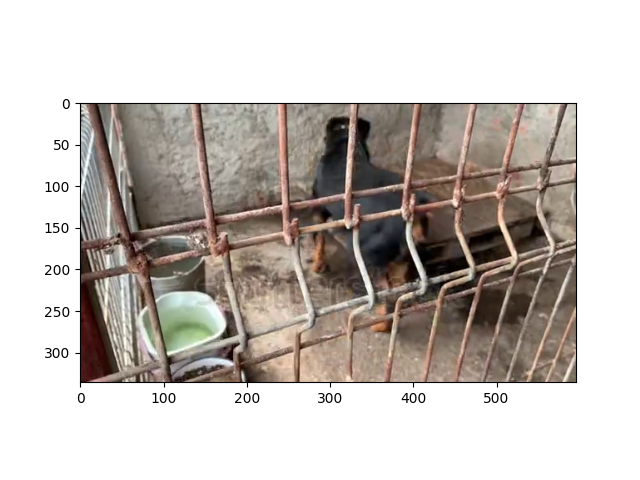
\includegraphics[width=0.45\textwidth]{figures/q_6_3_rot179.png}  &  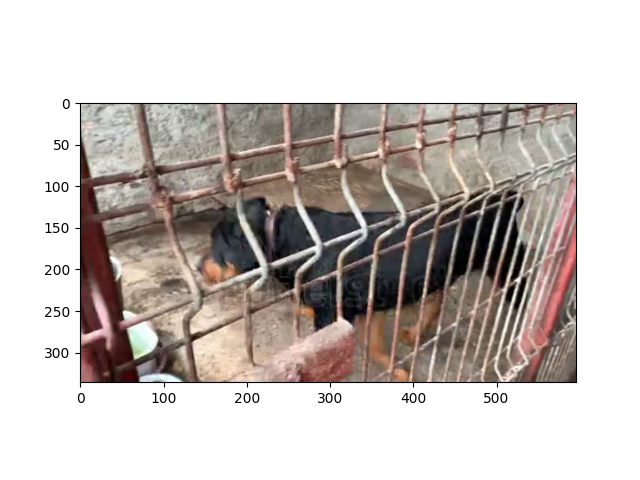
\includegraphics[width=0.45\textwidth]{figures/q_6_3_rot269.png}  \\  
    \textbf{(c)} Frame 180 & \textbf{(d)} Frame 270\\ [6pt] 

    \end{tabular}
    \caption{Frames 0, 90, 180 and 270 of the rotweiller video}\label{fig:q_6_3}
\end{figure} 

ResNet50 did not predict rotweiller for any of the 270 frames. However, interestingly enough, the three most commons predicted labels were: worm fence (39\%), prison (29.0\%) and steel arch bridge (13.7\%). Clearly, the pattern
of the dog's cage hugely influences the label prediction. I also looked the top-5 accuracy, but still none of the frames were classified as rotweiller. This shows how important is to have a diversified dataset. 
One way of improving the model is to do some additional training with data that includes dogs in different contexts (e.g. cages). This can be done with original images, but also with data augmentation transformations.

\end{document}

